	\begin{center}
		\section{计算几何}
	\end{center}

	\subsection{点线基础模板}

		以下是计算几何最底层的几个基础类型：符号判定 \texttt{sgn}、点 / 向量 \texttt{Point}（点和向量同一类型，向量当成「以原点为起点」的点）、叉乘 / 点乘、两点式直线 \texttt{Line}。\textbf{后续所有子节的代码都建立在这些定义之上}，每节顶部会以注释形式列出本节用到的依赖（具体实现见此处）。

		\textbf{类型约定}：坐标类型 \texttt{T} 只用 \texttt{ll} 或 \texttt{DB}。\texttt{Wide<T>} 把整数乘积（叉积、点积、模长平方）升为 \texttt{i128}，浮点保留原类型；坐标加减本身仍须落在 \texttt{T} 的范围内。\texttt{Promote} 让 \texttt{Point<ll>} 能隐式转成 \texttt{Point<DB>}，反向禁止。\texttt{+ - cross dot} 都只写同类型版本，混合类型表达式（如 \texttt{Point<ll> - Point<DB>}）靠这个隐式转换自动走 \texttt{DB} 版本；标量乘除 \texttt{p * k}、\texttt{p / k} 返回公共类型，所以 \texttt{Point<ll> / DB} 得到 \texttt{Point<DB>}，不会截断。\texttt{sqrtL} 对整数先精确开方再修正，避免 \texttt{i128} 转浮点丢精度。排序使用精确字典序，\texttt{eps} 只用于几何判定与 \texttt{==}，不能放进排序比较器。拷贝与类型转换保留 \texttt{id}，算术派生点的 \texttt{id=-1}。

		\href{https://gist.github.com/znzryb/11d094702ccdb989efb8aed573ab0885}{change log}

		% geometry-code: point-line
\begin{minted}{cpp}
// C++17；ll / i128 / DB / eps / PI 由开赛模板定义。坐标类型 T 只用 ll 或 DB。
// Wide：整数乘积升 i128 防溢出；Promote：只允许 Point<ll> -> Point<DB> 这种无损方向的隐式转换。
template<class T> using Wide = conditional_t<is_floating_point_v<T>, T, i128>;
template<class T, class U> using Promote = enable_if_t<is_same_v<common_type_t<T, U>, T>>;
template<class T> int sgn(T x) { return (x > eps) - (x < -eps); }
template<class T> Wide<T> squared(T x) { return Wide<T>(x) * x; }
DB sqrtL(DB x) { return sqrtl(x); }
DB sqrtL(i128 n) { // 整数先精确开方再修正，避免 i128 转浮点丢精度
	if (n <= 0) return 0;
	i128 s = sqrtl((DB)n);
	while (s * s > n) --s;
	while ((s + 1) * (s + 1) <= n) ++s;
	return s + (DB)(n - s * s) / (sqrtl((DB)n) + s);
}

template<class T>
struct Point {
	T x, y;
	int id = -1; // 拷贝 / 类型转换保留下标，算术派生点为 -1
	explicit Point(T x = 0, T y = 0) : x(x), y(y) {}
	template<class U, class = Promote<T, U>> Point(Point<U> p) : x(p.x), y(p.y), id(p.id) {}
	// 混合类型（ll 与 DB）运算靠隐式转换走 DB 版本；标量乘除返回公共类型，Point<ll> / DB 不会截断
	friend Point operator+(Point a, Point b) { return Point(a.x + b.x, a.y + b.y); }
	friend Point operator-(Point a, Point b) { return Point(a.x - b.x, a.y - b.y); }
	Point operator-() const { return Point(-x, -y); }
	template<class U> friend auto operator*(Point a, U k) { return Point<common_type_t<T, U>>(a.x * k, a.y * k); }
	template<class U> friend auto operator*(U k, Point a) { return a * k; }
	template<class U> friend auto operator/(Point a, U k) { return Point<common_type_t<T, U>>(a.x / k, a.y / k); }
	Point &operator+=(Point p) { return *this = *this + p; }
	Point &operator-=(Point p) { return *this = *this - p; }
	// 排序用精确字典序（eps 会破坏 strict weak ordering），== 才用 eps
	friend bool operator<(Point a, Point b) { return tie(a.x, a.y) < tie(b.x, b.y); }
	friend bool operator==(Point a, Point b) { return !sgn(a.x - b.x) && !sgn(a.y - b.y); }
	friend bool operator!=(Point a, Point b) { return !(a == b); }
	friend istream &operator>>(istream &s, Point &p) { return s >> p.x >> p.y; }
	friend ostream &operator<<(ostream &s, Point p) { return s << "(" << p.x << ", " << p.y << ")"; }
	friend Wide<T> cross(Point a, Point b) { return Wide<T>(a.x) * b.y - Wide<T>(a.y) * b.x; }
	friend Wide<T> dot(Point a, Point b) { return Wide<T>(a.x) * b.x + Wide<T>(a.y) * b.y; }
	friend Wide<T> cross(Point o, Point a, Point b) { return cross(a - o, b - o); } // 以 o 为原点
	friend Wide<T> dot(Point o, Point a, Point b) { return dot(a - o, b - o); }
	Wide<T> norm() const { return dot(*this, *this); } // 模长平方
	DB abs() const { return sqrtL(norm()); }
	Wide<T> normL1() const { return (Wide<T>)(x < 0 ? -x : x) + (y < 0 ? -y : y); }
	T normLinf() const { return max(x < 0 ? -x : x, y < 0 ? -y : y); }
	Point rot90() const { return Point(-y, x); }
	Point<DB> rot(DB a) const { return Point<DB>(x * cosl(a) - y * sinl(a), x * sinl(a) + y * cosl(a)); }
};

template<class T>
struct Line { // 直线 / 线段共用：p1 -> p2
	Point<T> p1, p2;
	Line(Point<T> a = Point<T>(), Point<T> b = Point<T>()) : p1(a), p2(b) {}
	Line(T k, T c) : p1(0, c), p2(1, k + c) {} // 斜截式 y = kx + c
	template<class U, class = Promote<T, U>> Line(Line<U> l) : p1(l.p1), p2(l.p2) {}
	friend bool operator<(Line a, Line b) { return tie(a.p1, a.p2) < tie(b.p1, b.p2); }
	friend bool operator==(Line a, Line b) { return a.p1 == b.p1 && a.p2 == b.p2; }
	friend istream &operator>>(istream &s, Line &l) { return s >> l.p1 >> l.p2; }
	friend ostream &operator<<(ostream &s, Line l) { return s << "<" << l.p1 << ", " << l.p2 << ">"; }
};
// 一般式 ax + by + c = 0（a、b 不同时为 0）
Line<DB> gen_line_from_general(DB a, DB b, DB c) {
	Point<DB> p = b != 0 ? Point<DB>(0, -c / b) : Point<DB>(-c / a, 0);
	return Line<DB>(p, p + Point<DB>(b, -a));
}
mt19937_64 rng(chrono::steady_clock::now().time_since_epoch().count());
\end{minted}

		\textbf{参考题单}：\href{https://vjudge.net/article/12247}{计算几何模板题目总结}（vjudge）以及 \href{https://qoj.ac/contest/2646}{QOJ 模板赛 2646}。

		\subsection{点在线上的投影点}

		\href{https://vjudge.net/solution/64166651}{vjudge 提交}。

		设 \texttt{vec = l.p2 - l.p1}，把向量 \texttt{p - l.p1} 在 \texttt{vec} 方向上的归一化投影长度记为 $r$，于是投影点等于 \texttt{l.p1 + r * vec}。\textbf{返回值固定为 \texttt{Point<DB>}}（除法走浮点，输入 \texttt{T / U} 是 \texttt{ll} 还是 \texttt{DB} 都向 \texttt{DB} 收敛），不再 \texttt{assert} 浮点。

		% geometry-code: projection
\begin{minted}{cpp}
// 依赖：点线基础；l 非退化。返回值固定为 Point<DB>
template<class T, class U>
Point<DB> project(Point<T> p, Line<U> l) {
	Point<DB> v = l.p2 - l.p1;
	return l.p1 + v * (dot(v, p - l.p1) / v.norm());
}
\end{minted}

		\subsection{对称点}

		\href{https://vjudge.net/solution/64168723}{vjudge 提交}。

		设 \texttt{proj} 为投影点，则对称点 \texttt{= proj + proj - p}。直观上：\textcolor{blue}{\textbf{以投影点为中点}}，原点和对称点处于直线两侧、距离相等。

		\begin{center}
			\begin{tikzpicture}[>=Stealth]
				\draw[thick, blue!70!black] (-2.2, 0) -- (2.6, 0) node[right, font=\scriptsize] {$L$};
				\coordinate (P)  at (0.5,  1.4);
				\coordinate (Pp) at (0.5,  0);
				\coordinate (Pr) at (0.5, -1.4);
				\draw[dashed, gray] (P) -- (Pr);
				\draw[gray] (0.3, 0) -- (0.3, 0.2) -- (0.5, 0.2);
				\fill[red]    (P)  circle (1.8pt) node[above right, font=\scriptsize, color=red]    {$P$};
				\fill[teal]   (Pp) circle (1.8pt) node[above left,  font=\scriptsize, color=teal]   {$P'$ (proj)};
				\fill[orange] (Pr) circle (1.8pt) node[below right, font=\scriptsize, color=orange] {$P''$};
				\draw[<->, blue!50!black, thin] (-1.5, 0.05) -- (-1.5, 1.35) node[midway, left, font=\tiny] {$d$};
				\draw[<->, blue!50!black, thin] (-1.5, -0.05) -- (-1.5, -1.35) node[midway, left, font=\tiny] {$d$};
			\end{tikzpicture}

			\vspace{2pt}
			{\footnotesize\sffamily\color{gray} 图注：$P'$（投影）是 $P$ 到 $L$ 的垂足；$P''$（对称点）满足 $P'$ 是 $P, P''$ 中点，从而 $P'' = 2P' - P$。}
		\end{center}

		% geometry-code: reflection
\begin{minted}{cpp}
// 依赖：project
template<class T, class U>
Point<DB> reflect(Point<T> p, Line<U> l) { return project(p, l) * 2 - p; }
\end{minted}

		\subsection{点线位置判断（CCW）}

		\href{https://vjudge.net/solution/64174955}{vjudge 提交}。

		给一条有向直线 $\overrightarrow{a \to b}$，目标点 $p$ 落在何处由 $\mathrm{cross}(\vec{ab}, \vec{ap})$ 与 $\mathrm{dot}(\vec{ab}, \vec{ap})$ 决定，共五种情况：

		\begin{center}
			\begin{tikzpicture}[>=Stealth, x=1cm, y=1cm]
				\begin{scope}
					\draw[->, thick] (0,0) -- (1.2,0);
					\fill (0,0) circle (1pt); \fill (1.2,0) circle (1pt);
					\fill[teal] (0.6, 0.5) circle (1.6pt) node[above, font=\tiny, color=teal] {$p$};
					\node[font=\tiny, anchor=north] at (0.6, -0.55) {COUNTER\_CCW};
				\end{scope}
				\begin{scope}[xshift=2.4cm]
					\draw[->, thick] (0,0) -- (1.2,0);
					\fill (0,0) circle (1pt); \fill (1.2,0) circle (1pt);
					\fill[orange] (0.6, -0.5) circle (1.6pt) node[below, font=\tiny, color=orange] {$p$};
					\node[font=\tiny, anchor=north] at (0.6, -0.85) {CLOCKWISE};
				\end{scope}
				\begin{scope}[xshift=4.8cm]
					\draw[->, thick] (0,0) -- (1.2,0);
					\fill (0,0) circle (1pt); \fill (1.2,0) circle (1pt);
					\fill[violet] (-0.5, 0) circle (1.6pt) node[above, font=\tiny, color=violet] {$p$};
					\node[font=\tiny, anchor=north] at (0.35, -0.55) {ONLINE\_BACK};
				\end{scope}

				\begin{scope}[yshift=-2.0cm]
					\draw[->, thick] (0,0) -- (1.2,0);
					\fill (0,0) circle (1pt); \fill (1.2,0) circle (1pt);
					\fill[red] (1.7, 0) circle (1.6pt) node[above, font=\tiny, color=red] {$p$};
					\node[font=\tiny, anchor=north] at (0.85, -0.55) {ONLINE\_FRONT};
				\end{scope}
				\begin{scope}[xshift=2.4cm, yshift=-2.0cm]
					\draw[->, thick] (0,0) -- (1.2,0);
					\fill (0,0) circle (1pt); \fill (1.2,0) circle (1pt);
					\fill[blue] (0.6, 0) circle (1.6pt) node[above, font=\tiny, color=blue] {$p$};
					\node[font=\tiny, anchor=north] at (0.6, -0.55) {ON\_SEGMENT};
				\end{scope}
				\node[font=\tiny] at (0, 0.18) {$a$};
				\node[font=\tiny] at (1.2, 0.18) {$b$};
			\end{tikzpicture}

			\vspace{2pt}
			{\footnotesize\sffamily\color{gray} 图注：先看 $\mathrm{cross}(\vec{ab},\vec{ap})$ 的符号——正左 / 负右；为零再看 $\mathrm{dot}$ 与 $|\vec{ab}|, |\vec{ap}|$ 的比较，区分 $p$ 落在线段反方向延长（BACK）、正方向延长（FRONT）还是线段内部（ON）。}
		\end{center}

		% geometry-code: ccw
\begin{minted}{cpp}
// 依赖：点线基础
constexpr int ON_SEGMENT = 0, COUNTER_CLOCKWISE = 1, CLOCKWISE = -1, ONLINE_BACK = 2, ONLINE_FRONT = -2;
template<class T, class U>
int CCW(Point<T> p, Line<U> l) {
	auto a = l.p2 - l.p1; auto b = p - l.p1;
	if (int s = sgn(cross(a, b))) return s;
	if (sgn(dot(a, b)) < 0) return ONLINE_BACK;
	return a.norm() < b.norm() ? ONLINE_FRONT : ON_SEGMENT;
}
\end{minted}

		\subsubsection{逆时针弧角 \texttt{ccw\_angle}（标量 / 向量两版）}

		求「从 \texttt{from} 逆时针转到 \texttt{to}」的有向夹角，结果恒落在 $[0, 2\pi)$，而不是 $|\texttt{to} - \texttt{from}|$（后者在跨 $0/2\pi$ 处会算错）。两个重载：标量版输入两个极角，向量版输入两个方向向量、用单次 $\operatorname{atan2}(\mathrm{cross}, \mathrm{dot})$（叉积当 $\sin$ 分量、点积当 $\cos$ 分量）一步求出，比两次 \texttt{atan2} 相减更稳。

		% geometry-code: ccw-angle
\begin{minted}{cpp}
// 依赖：点线基础。从 from 逆时针转到 to 的角，落在 [0, 2pi)，不是 abs(to - from)
DB ccw_angle(DB from, DB to) {
	DB d = fmodl(to - from, 2 * PI);
	return d < 0 ? d + 2 * PI : d;
}
template<class T, class U> // 向量版：单次 atan2(cross, dot) 比两次 atan2 相减稳
DB ccw_angle(Point<T> from, Point<U> to) {
	DB d = atan2l(cross(from, to), dot(from, to));
	return d < 0 ? d + 2 * PI : d;
}
\end{minted}

		\subsection{判断两直线是否垂直 / 平行}

		\href{https://vjudge.net/solution/64175524}{vjudge 提交}。

		分别取两条直线的方向向量，看 \texttt{dot} 是否为零（垂直）或 \texttt{cross} 是否为零（平行）。

		% geometry-code: orthogonal-parallel
\begin{minted}{cpp}
// 依赖：点线基础
template<class T, class U> bool isOrthogonal(Line<T> a, Line<U> b) { return !sgn(dot(a.p2 - a.p1, b.p2 - b.p1)); }
template<class T, class U> bool isParallel(Line<T> a, Line<U> b) { return !sgn(cross(a.p2 - a.p1, b.p2 - b.p1)); }
\end{minted}

		\subsection{判断两线段是否相交}

		\href{https://vjudge.net/solution/64175810}{vjudge 提交}。

		\texttt{a} 与 \texttt{b} 相交当且仅当 \texttt{b} 的两端点关于 \texttt{a} 异侧（含端点重合）\textbf{且} \texttt{a} 的两端点关于 \texttt{b} 异侧。利用 \texttt{CCW} 的符号相乘 $\le 0$ 即可。

		% geometry-code: segment-intersection
\begin{minted}{cpp}
// 依赖：CCW；含端点相交与退化为点的线段
template<class T, class U>
bool isSegIntersect(Line<T> a, Line<U> b) {
	if (a.p1 == a.p2) return CCW(a.p1, b) == ON_SEGMENT;
	if (b.p1 == b.p2) return CCW(b.p1, a) == ON_SEGMENT;
	return CCW(b.p1, a) * CCW(b.p2, a) <= 0 && CCW(a.p1, b) * CCW(a.p2, b) <= 0;
}
\end{minted}

		\textbf{命名提示}：函数名特意叫 \texttt{isSegIntersect}（不是 \texttt{isIntersect}）——\texttt{Line<T>} 在本模板里同时承担「直线」与「线段」两种语义，这里 \texttt{a, b} 是被当成线段判定的，函数名前加 \texttt{Seg} 防止与「两\textbf{直线}是否相交」（任意非平行直线都相交）混淆。

		\subsection{两条直线交点}

		\href{https://vjudge.net/solution/64186810}{vjudge 提交}。

		设两条直线分别用方向式 $p + t\vec{v}$、$q + s\vec{w}$。在交点处：
		\begin{align*}
			p + t\vec{v} &= q + s\vec{w} \\
			(p - q) \times \vec{w} + t\, \vec{v} \times \vec{w} &= 0 \quad (\text{两边叉乘 } \vec{w}\text{，自身叉乘消去 } s\vec{w}) \\
			t &= \dfrac{\vec{w} \times (p - q)}{\vec{v} \times \vec{w}}
		\end{align*}
		交点即 $p + t\vec{v}$。\textbf{返回值固定为 \texttt{Point<DB>}}（除法走浮点，不论输入 \texttt{T} 是什么都向 \texttt{DB} 收敛）。函数体内先把所有 \texttt{Point<T>} 走 promotion 提到 \texttt{Point<DB>}，整数 \texttt{T} 也合法（实参为整数 \texttt{Line<ll>} 时不再 \texttt{assert}）。

		% geometry-code: line-intersection
\begin{minted}{cpp}
// 依赖：点线基础；两条非退化、不平行直线。返回值固定为 Point<DB>
template<class T, class U>
Point<DB> getintersect(Line<T> a, Line<U> b) {
	Point<DB> p = a.p1, v = a.p2 - a.p1, q = b.p1, w = b.p2 - b.p1;
	return p + v * (cross(w, p - q) / cross(v, w));
}
\end{minted}

		\subsection{两线段间最小距离}

		\href{https://vjudge.net/solution/64187931}{vjudge 提交}。

		若两线段相交则距离为 $0$；否则取四个「端点 → 对方线段」距离的最小值。点到线段距离 \texttt{distancePS} 中要先判断投影是否落在线段两端之外，落到外面就退化为对应端点的距离。

		% geometry-code: distances
\begin{minted}{cpp}
// 依赖：CCW, isSegIntersect。PPNorm 是距离平方（不开方，留到最后再 sqrt）；L1 / Linf 返回坐标公共类型
template<class T, class U> auto distancePPNorm(Point<T> a, Point<U> b) { return (a - b).norm(); }
template<class T, class U> DB distancePP(Point<T> a, Point<U> b) { return (a - b).abs(); }
template<class T, class U> auto distancePPL1(Point<T> a, Point<U> b) { return (a - b).normL1(); }
template<class T, class U> auto distancePPLinf(Point<T> a, Point<U> b) { return (a - b).normLinf(); }
template<class T, class U>
DB distancePL(Point<T> p, Line<U> l) { // 点到直线
	auto v = cross(l.p1, l.p2, p);
	return (v < 0 ? -v : v) / (l.p2 - l.p1).abs();
}
template<class T, class U>
DB distancePS(Point<T> p, Line<U> l) { // 点到线段，AC https://qoj.ac/submission/2001668
	if (l.p1 == l.p2) return (p - l.p1).abs();
	if (sgn(dot(l.p2 - l.p1, p - l.p1)) < 0) return (p - l.p1).abs();
	if (sgn(dot(l.p1 - l.p2, p - l.p2)) < 0) return (p - l.p2).abs();
	return distancePL(p, l);
}
template<class T, class U>
DB distanceSS(Line<T> a, Line<U> b) { // 线段到线段，AC https://qoj.ac/submission/2001588
	if (isSegIntersect(a, b)) return 0;
	return min({distancePS(a.p1, b), distancePS(a.p2, b), distancePS(b.p1, a), distancePS(b.p2, a)});
}
\end{minted}

		\subsection{多边形面积}

		\href{https://vjudge.net/solution/64207564}{vjudge 提交}。

		用「向量叉乘求三角形有向面积之和」（鞋带公式）：
		$$
		A = \frac{1}{2} \left| \sum_{i=0}^{n-1} \mathrm{cross}(P_i, P_{(i+1) \bmod n}) \right|
		$$
		逆时针排列时 $\sum$ 本身已为正，顺时针为负，统一取绝对值。

		\textbf{拆出 \texttt{polygonSignedArea}}：返回值 \texttt{Wide<T>} 跟着 \texttt{cross} 走（整数 \texttt{T} $\to$ \texttt{i128}，浮点 \texttt{T} $\to$ \texttt{T}）。\textcolor{red}{\textbf{不要}}像旧版那样写成 \texttt{DB res = 0; res += cross(...)}——在整数 \texttt{T} 下 \texttt{cross} 返回 \texttt{\_\_int128\_t}，赋给 \texttt{double} 累加器会在 $|val| > 2^{53}$ 时丢精度。除此之外，\texttt{reorder\_polygon} 也复用 \texttt{polygonSignedArea} 取符号判方向，避免「前三点共线」时的局部退化。

		% geometry-code: polygon-area
\begin{minted}{cpp}
// 依赖：点线基础。2 倍有向面积（> 0 CCW，< 0 CW，0 退化）；整数返回 i128，不丢精度
template<class T>
Wide<T> polygonSignedArea(const vector<Point<T>> &poly) {
	Wide<T> res = 0;
	int n = poly.size();
	for (int i = 0; i < n; ++i) res += cross(poly[i], poly[(i + 1) % n]);
	return res;
}
template<class T>
DB polygonArea(const vector<Point<T>> &poly) {
	auto s = polygonSignedArea(poly);
	return (DB)(s < 0 ? -s : s) / 2;
}
\end{minted}

% geometry-code: polygon-perimeter
\begin{minted}{cpp}
template<class T>
DB polygon_perimeter(const vector<Point<T>> &poly) {
	DB res = 0;
	int n = poly.size();
	for (int i = 0; i < n; ++i) res += (poly[i] - poly[(i + 1) % n]).abs();
	return res;
}
\end{minted}

% geometry-code: regular-polygon
\begin{minted}{cpp}
// 正 n 边形面积 A = n l^2 / (4 tan(pi / n))，n >= 3
DB regular_polygon_area(ll n, DB l) { return n * l * l / (4 * tanl(PI / n)); }
\end{minted}

		\subsection{圆 \texttt{Circle}：测度五件套}

		圆心 \texttt{c} + 半径 \texttt{r} 的最小描述，配套\textbf{弧长 / 弦长 / 弓形高 / 扇形面积 / 弓形面积}五件套测度。

		\textbf{角度约定}：入参 \texttt{theta} 是弦所对的\textbf{圆心角}，单位\textbf{弧度}，约束 $\theta \in [0, 2\pi]$。$\theta < \pi$ 是 minor 弓形（小的那块），$\theta > \pi$ 是 major 弓形（大的那块），公式同一个，\textbf{不做内部 deg $\leftrightarrow$ rad 转换}（调用方自己 \texttt{deg * PI / 180}）。\texttt{point\_at} 接受任意 \texttt{theta}（含负值 / 超 $2\pi$），不抛 assert——绕圆走多圈合法。

		\textbf{\texttt{theta\_at}：\texttt{point\_at} 的逆}：给定圆上一点 $p$，返回它相对圆心的极角。\texttt{atan2l} 出来的是 $(-\pi, \pi]$，加一次 $2\pi$ 归一化到 $[0, 2\pi)$，于是 $\texttt{point\_at}(\texttt{theta\_at}(p)) = p$（$p$ 在圆上时）。不检查 $p$ 是否真在圆上，由调用方保证。典型用法：把圆上若干交点转成极角后排序，扫出相邻弧段。

		\texttt{point\_at} 直接用标准 \texttt{cosl/sinl}，不绑定编译器专有的 \texttt{sincos} 指针类型；\texttt{DB} 采用 \texttt{double} 或 \texttt{long double} 都能编译。

		\textbf{弓形面积公式}：弓形 = 扇形 $-$ 三角形，化简得
		$$S_{\text{seg}}(\theta) = \tfrac{1}{2} r^2 (\theta - \sin \theta).$$
		AC 实战：\href{https://vjudge.net/problem/Gym-105161B}{Gym 105161B Area of the Devil}（圆 $-$ 五块 segment $-$ 五块三角形）。

		\textbf{\texttt{ccw\_angle} helper}：从极角 \texttt{theta\_from} CCW 转到 \texttt{theta\_to} 的弧度差，落在 $[0, 2\pi)$。\textcolor{red}{\textbf{不要}}用 \texttt{abs(theta\_to - theta\_from)}——后者在 wrap 处（例如 from $= 352^{\circ}$, to $= 54^{\circ}$）会算成 $298^{\circ}$ 而非真实的 $62^{\circ}$。

		% geometry-code: circle
\begin{minted}{cpp}
// enum 值即两圆公切线条数；COINCIDENT = -1 表示重合（无穷多）
enum CircleRelation { COINCIDENT = -1, ONE_CONTAINS_OTHER, INTERNALLY_TANGENT, INTERSECTING, EXTERNALLY_TANGENT, EXTERNALLY_APART };

// 依赖：点线基础, distancePPNorm。theta 均为弧度制圆心角
template<class T>
struct Circle {
	Point<T> c; T r;
	explicit Circle(Point<T> c = Point<T>(), T r = 0) : c(c), r(r) {}
	template<class U, class = Promote<T, U>> Circle(Circle<U> o) : c(o.c), r(o.r) {}
	Point<DB> point_at(DB t) const { return c + Point<DB>(cosl(t), sinl(t)) * (DB)r; } // 极角 t 处的点，t 不限范围
	template<class U> DB theta_at(Point<U> p) const { // point_at 的逆：圆上点 p 的极角，[0, 2pi)
		Point<DB> d = p - c;
		DB t = atan2l(d.y, d.x);
		return t < 0 ? t + 2 * PI : t;
	}
	DB arc_length(DB t) const { return r * t; }
	DB chord_length(DB t) const { return 2 * r * sinl(t / 2); }
	DB sagitta(DB t) const { return r * (1 - cosl(t / 2)); } // 弓形高
	DB sector_area(DB t) const { return (DB)r * r * t / 2; }
	DB segment_area(DB t) const { return (DB)r * r * (t - sinl(t)) / 2; } // 弓形 = 扇形 - 三角形
	template<class U> bool is_point_in_circle(Point<U> p) const { return sgn(distancePPNorm(p, c) - squared(r)) <= 0; }
	friend istream &operator>>(istream &s, Circle &a) { return s >> a.c >> a.r; }
	friend ostream &operator<<(ostream &s, Circle a) { return s << "<" << a.c << "," << a.r << ">"; }
};
Circle<DB> circle_from_diameter(Point<DB> a, Point<DB> b) { return Circle<DB>((a + b) / 2, distancePP(a, b) / 2); }
\end{minted}

		\subsection{两圆位置关系 \texttt{circle\_relation}}

		\href{https://vjudge.net/solution/69918813}{vjudge 提交}（\href{https://vjudge.net/problem/Aizu-CGL_7_A}{Aizu CGL\_7\_A}）。

		按圆心距 $d$ 与 $r_1 \pm r_2$ 的关系判 5 种位置：相离 / 外切 / 相交 / 内切 / 内含。\textbf{enum 取值即两圆公切线条数}（外离 4 / 外切 3 / 相交 2 / 内切 1 / 内含 0），方便直接拿来当答案输出。

		\textbf{重合圆 sentinel \texttt{COINCIDENT = -1}}：同心同径时公切线无穷多，单独一档；调用方按需特判（如题面要求输出 \texttt{-1} / \texttt{Inf} / 任意大数）。

		\textbf{用 $\mathrm{squared}(d)$ 与 $\mathrm{squared}(r_1 \pm r_2)$ 比较，不直接比 $d$}：整数情形 $(r_1 + r_2)^2$ 在 \texttt{ll} 边界（输入 1e9 量级）会溢，走 \texttt{squared()} 自动升 \texttt{\_\_int128\_t} 防溢出；浮点情形也省一次 \texttt{sqrt}。

		% geometry-code: circle-relation
\begin{minted}{cpp}
// 依赖：Circle。全程平方比较，不开方
template<class T>
CircleRelation circle_relation(Circle<T> a, Circle<T> b) {
	auto d2 = distancePPNorm(a.c, b.c);
	if (!sgn(d2) && !sgn(a.r - b.r)) return COINCIDENT;
	int o = sgn(d2 - squared(a.r + b.r)), i = sgn(d2 - squared(a.r - b.r));
	if (o > 0) return EXTERNALLY_APART;
	if (o == 0) return EXTERNALLY_TANGENT;
	return i > 0 ? INTERSECTING : i == 0 ? INTERNALLY_TANGENT : ONE_CONTAINS_OTHER;
}
\end{minted}

		\subsection{三角形内接圆 / 外接圆}

		\textbf{内接圆 \texttt{incircle\_triangle}}：\href{https://vjudge.net/solution/69920478}{vjudge 提交}（\href{https://vjudge.net/problem/Aizu-CGL_7_B}{Aizu CGL\_7\_B}）。内心 $I$ 是三条\textbf{角平分线}的交点，用重心式直接写出：
		$$I = \frac{|BC| \cdot A + |AC| \cdot B + |AB| \cdot C}{|AB| + |AC| + |BC|}.$$
		内切圆半径 $r = $ 内心到任意一条边的距离，取 \texttt{min} 三条边距离做防御性数值兜底（三个值理论上相等，浮点下取最小避免 r 越界出三角形）。

		\textbf{外接圆 \texttt{outcircle\_triangle}}：\href{https://vjudge.net/solution/69927652}{vjudge 提交}（\href{https://vjudge.net/problem/Aizu-CGL_7_C}{Aizu CGL\_7\_C}）。外心 $O$ 是三条\textbf{垂直平分线}的交点，取 $AB$ 与 $AC$ 两边的中垂线求交即可：
		\begin{itemize}
			\setlength\itemsep{0pt}
			\item $AB$ 中点 $M_{AB} = (A + B) / 2$，中垂线方向 $= (B - A)$\texttt{.rot90()}；
			\item $AC$ 中点 $M_{AC} = (A + C) / 2$，中垂线方向 $= (C - A)$\texttt{.rot90()}；
			\item $O = \texttt{getintersect}(L_{AB}, L_{AC})$，$R = |O - A|$。
		\end{itemize}

		\textcolor{red}{\textbf{不要}}用「重心式」($I = (a \cdot BC + b \cdot AC + c \cdot AB)/(AB+AC+BC)$）求外心——那是\textbf{内心}公式，等腰 / 等边三角形样例下两者重合，会侥幸过样例但 WA。

		\textbf{退化 sentinel}：三点共线 / 任意两点重合（\texttt{cross(a, b, c) == 0}）时，内接圆 / 外接圆都不存在，分别返 \texttt{r = 0} 与 \texttt{r = -1} 作 sentinel；调用方用 \texttt{ci.r == 0} / \texttt{co.r < 0} 判退化即可，不会再吃到除零 NaN。

		% geometry-code: triangle-circles
\begin{minted}{cpp}
// 依赖：Circle, distancePP, getintersect。三点共线 / 重合时：内接圆返回 r = 0，外接圆返回 r = -1
Circle<DB> incircle_triangle(Point<DB> a, Point<DB> b, Point<DB> c) {
	DB s = cross(a, b, c);
	if (!sgn(s)) return Circle<DB>(a, 0);
	DB ab = distancePP(a, b), ac = distancePP(a, c), bc = distancePP(b, c), p = ab + ac + bc;
	return Circle<DB>((a * bc + b * ac + c * ab) / p, (s < 0 ? -s : s) / p);
}
Circle<DB> outcircle_triangle(Point<DB> a, Point<DB> b, Point<DB> c) { // 两条中垂线的交点
	if (!sgn(cross(a, b, c))) return Circle<DB>(a, -1);
	Point<DB> m1 = (a + b) / 2, m2 = (a + c) / 2;
	Point<DB> o = getintersect(Line(m1, m1 + (b - a).rot90()), Line(m2, m2 + (c - a).rot90()));
	return Circle<DB>(o, distancePP(o, a));
}
\end{minted}

		\subsection{直线与圆的关系 / 交点 \texttt{circle\_line\_relation} / \texttt{getCrossPointsCL}}

		\href{https://vjudge.net/solution/69928470}{vjudge 提交}（\href{https://vjudge.net/problem/Aizu-CGL_7_D}{Aizu CGL\_7\_D}）；弦长版 \href{https://vjudge.net/solution/69929454}{vjudge 提交}（\href{https://vjudge.net/problem/EOlymp-359}{EOlymp-359}）。

		\textbf{关系判定}：圆心 $C$ 到直线距离 $d = |\mathrm{cross}(p_1, p_2, C)| / |p_2 - p_1|$，与半径 $r$ 比较。两边平方 + 乘 $|p_2 - p_1|^2$ 走整数：$\mathrm{cross}^2$ vs $r^2 \cdot |p_2 - p_1|^2$，\texttt{squared()} 自动升 \texttt{\_\_int128\_t} 防溢。

		\textbf{交点求法}：先取垂足 $F = \mathrm{project}(C, l)$，半弦长 $h = \sqrt{r^2 - |CF|^2}$（斜边 $r$ 与直角边 $|CF|$ 在直角三角形里推另一直角边），单位方向 $\hat{d} = (p_2 - p_1) / |p_2 - p_1|$，交点 $F \pm \hat{d} \cdot h$。

		\textbf{退化 sentinel}：\texttt{l.p1 == l.p2} 时直接返 0 / 空集，不会跑到 \texttt{project} 的除零路径。

		% geometry-code: circle-line
\begin{minted}{cpp}
// 依赖：Circle, project。关系：0 相离 / 1 相切 / 2 相交；退化直线视为无交点
template<class T>
int circle_line_relation(Circle<T> cir, Line<T> l) {
	if (l.p1 == l.p2) return 0;
	return 1 - sgn(squared(cross(l.p1, l.p2, cir.c)) - squared(cir.r) * (l.p2 - l.p1).norm());
}
template<class T>
vector<Point<DB>> getCrossPointsCL(Circle<T> cir, Line<T> l) {
	int k = circle_line_relation(cir, l);
	if (!k) return {};
	Point<DB> f = project(cir.c, l), d = l.p2 - l.p1; // 垂足 f，沿 l 方向 +- 半弦长
	if (k == 1) return {f};
	d = d / d.abs() * (DB)sqrtl(max((DB)0, (DB)cir.r * cir.r - (cir.c - f).norm()));
	return {f - d, f + d};
}
\end{minted}

		\subsection{线段与圆的关系 / 交点 \texttt{circle\_segment\_relation} / \texttt{getCrossPointsCS}}

		\textbf{为什么要单独一份}：\texttt{Line<T>} 在本模板里同时当直线与线段用，而上面的 \texttt{getCrossPointsCL} 是\textbf{直线}语义——交点可能落在 $p_1 p_2$ 之外的延长线上。线段版只需在直线版的结果上筛掉段外的交点：交点 $P$ 已经在直线上，所以「$P$ 落在线段内」等价于 $\mathrm{dot}(A - P,\, B - P) \le 0$（$P$ 看向两个端点的方向相反，$= 0$ 即 $P$ 就是某个端点）。

		\begin{center}
			\begin{tikzpicture}[>=Stealth, font=\scriptsize]
				% 返回 2：线段横穿圆
				\begin{scope}
					\draw[thick] (0,0) circle (0.9);
					\fill (0,0) circle (0.7pt);
					\draw[thick, red] (-1.4,0.35) -- (1.4,0.35);
					\fill[red] (-0.829,0.35) circle (1.2pt) (0.829,0.35) circle (1.2pt);
					\node[anchor=north, text width=2.4cm, align=center] at (0,-1.1) {返回 \texttt{2}\\两端都在圆外、横穿};
				\end{scope}
				% 返回 1：一端在圆内
				\begin{scope}[xshift=2.7cm]
					\draw[thick] (0,0) circle (0.9);
					\fill (0,0) circle (0.7pt);
					\draw[thick, orange] (0,-0.1) -- (1.5,-0.55);
					\fill[orange] (0.829,-0.349) circle (1.2pt);
					\node[anchor=north, text width=2.4cm, align=center] at (0,-1.1) {返回 \texttt{1}\\一端在圆内、穿出一次};
				\end{scope}
				% 返回 0：整段在圆内
				\begin{scope}[xshift=5.4cm]
					\draw[thick] (0,0) circle (0.9);
					\fill (0,0) circle (0.7pt);
					\draw[thick, blue] (-0.55,0.35) -- (0.5,-0.2);
					\node[anchor=north, text width=2.4cm, align=center] at (0,-1.1) {返回 \texttt{0}\\整段在圆内（与圆盘相交）};
				\end{scope}
				% 返回 0：只有延长线与圆相交
				\begin{scope}[xshift=8.4cm]
					\draw[thick] (0,0) circle (0.9);
					\fill (0,0) circle (0.7pt);
					\draw[thick, teal] (-1.5,-0.708) -- (-1.3,-0.635);
					\draw[teal, dashed] (-1.3,-0.635) -- (-0.43,-0.316);
					\draw[teal, fill=white] (-0.782,-0.445) circle (1.5pt);
					\node[anchor=north, text width=2.4cm, align=center] at (0,-1.1) {返回 \texttt{0}\\只有延长线相交};
				\end{scope}
			\end{tikzpicture}

			\vspace{2pt}
			{\footnotesize\sffamily\color{gray} 图注：四种情形下 \texttt{circle\_segment\_relation} 的返回值。右边两种 \texttt{getCrossPointsCL} 会分别给出 2 个交点（第四图中的空心点在延长线上）和 0 个交点，线段版都返回 0——这正是两者的差别。}
		\end{center}

		\textbf{返回值语义}：\texttt{circle\_segment\_relation} 返回\textbf{线段与圆周的公共点个数} $0 / 1 / 2$，与 \texttt{getCrossPointsCS} 给出的交点个数恒等。它跟直线版的「0 相离 / 1 相切 / 2 相交」\textcolor{red}{\textbf{不是一回事}}：
		\begin{itemize}
			\setlength\itemsep{0pt}
			\item 返回 0 可能是整段在圆外，也可能是\textbf{整段在圆内}（与圆盘相交，只是不穿过圆周）；
			\item 返回 1 可能是真相切，也可能是一端在圆内、一端在圆外只穿出一次。
		\end{itemize}
		要判「线段与\textbf{圆盘}有没有公共点」，用 \texttt{sgn(distancePS(cir.c, s) - cir.r) <= 0}（点到线段距离 $\le r$），别拿本函数的返回值当它用。

		\textbf{退化}：线段退化成一点（\texttt{s.p1 == s.p2}）时沿用直线版口径返回 0 / 空集，哪怕这个点正好落在圆周上。

		% geometry-code: circle-segment
\begin{minted}{cpp}
// 依赖：getCrossPointsCL。线段语义：只保留落在 s 内部（含端点）的交点
template<class T>
vector<Point<DB>> getCrossPointsCS(Circle<T> cir, Line<T> s) {
	vector<Point<DB>> res;
	for (Point<DB> p : getCrossPointsCL(cir, s))
		if (sgn(dot(s.p1 - p, s.p2 - p)) <= 0) res.push_back(p);
	return res;
}
// 线段与圆周的公共点个数 0 / 1 / 2；整段在圆内也返回 0，判与圆盘相交用 distancePS <= r
template<class T>
int circle_segment_relation(Circle<T> cir, Line<T> s) { return getCrossPointsCS(cir, s).size(); }
\end{minted}

		\subsection{两圆的关系 / 交点 \texttt{circle\_circle\_relation} / \texttt{getCrossPointsCC}}

		\href{https://vjudge.net/solution/69929473}{vjudge 提交}（\href{https://vjudge.net/problem/Aizu-CGL_7_E}{Aizu CGL\_7\_E}）；含重合 sentinel 版 \href{https://vjudge.net/solution/69929406}{vjudge 提交}（\href{https://vjudge.net/problem/EOlymp-4779}{EOlymp-4779}）。

		\textbf{关系判定}：$d^2$、$(r_1 + r_2)^2$、$(r_1 - r_2)^2$ 全走整数 \texttt{squared} 比较，不开方。$d^2 > (r_1 + r_2)^2$ 相离；$d^2 = (r_1 + r_2)^2$ 外切；$(r_1 - r_2)^2 < d^2 < (r_1 + r_2)^2$ 相交；$d^2 = (r_1 - r_2)^2$ 内切；$d^2 < (r_1 - r_2)^2$ 内含。

		\textbf{交点求法}：连心线方向 $\hat{d} = (c_2.c - c_1.c) / D$。弦中点 $M = c_1.c + \hat{d} \cdot a$，其中 $a = (r_1^2 - r_2^2 + D^2) / (2 D)$（联立两圆方程相减消平方项得到）。沿连心线垂直方向 $\hat{d}.\mathrm{rot90}()$ $\pm$ 半弦长 $h = \sqrt{r_1^2 - a^2}$ 即两交点。

		\begin{center}
			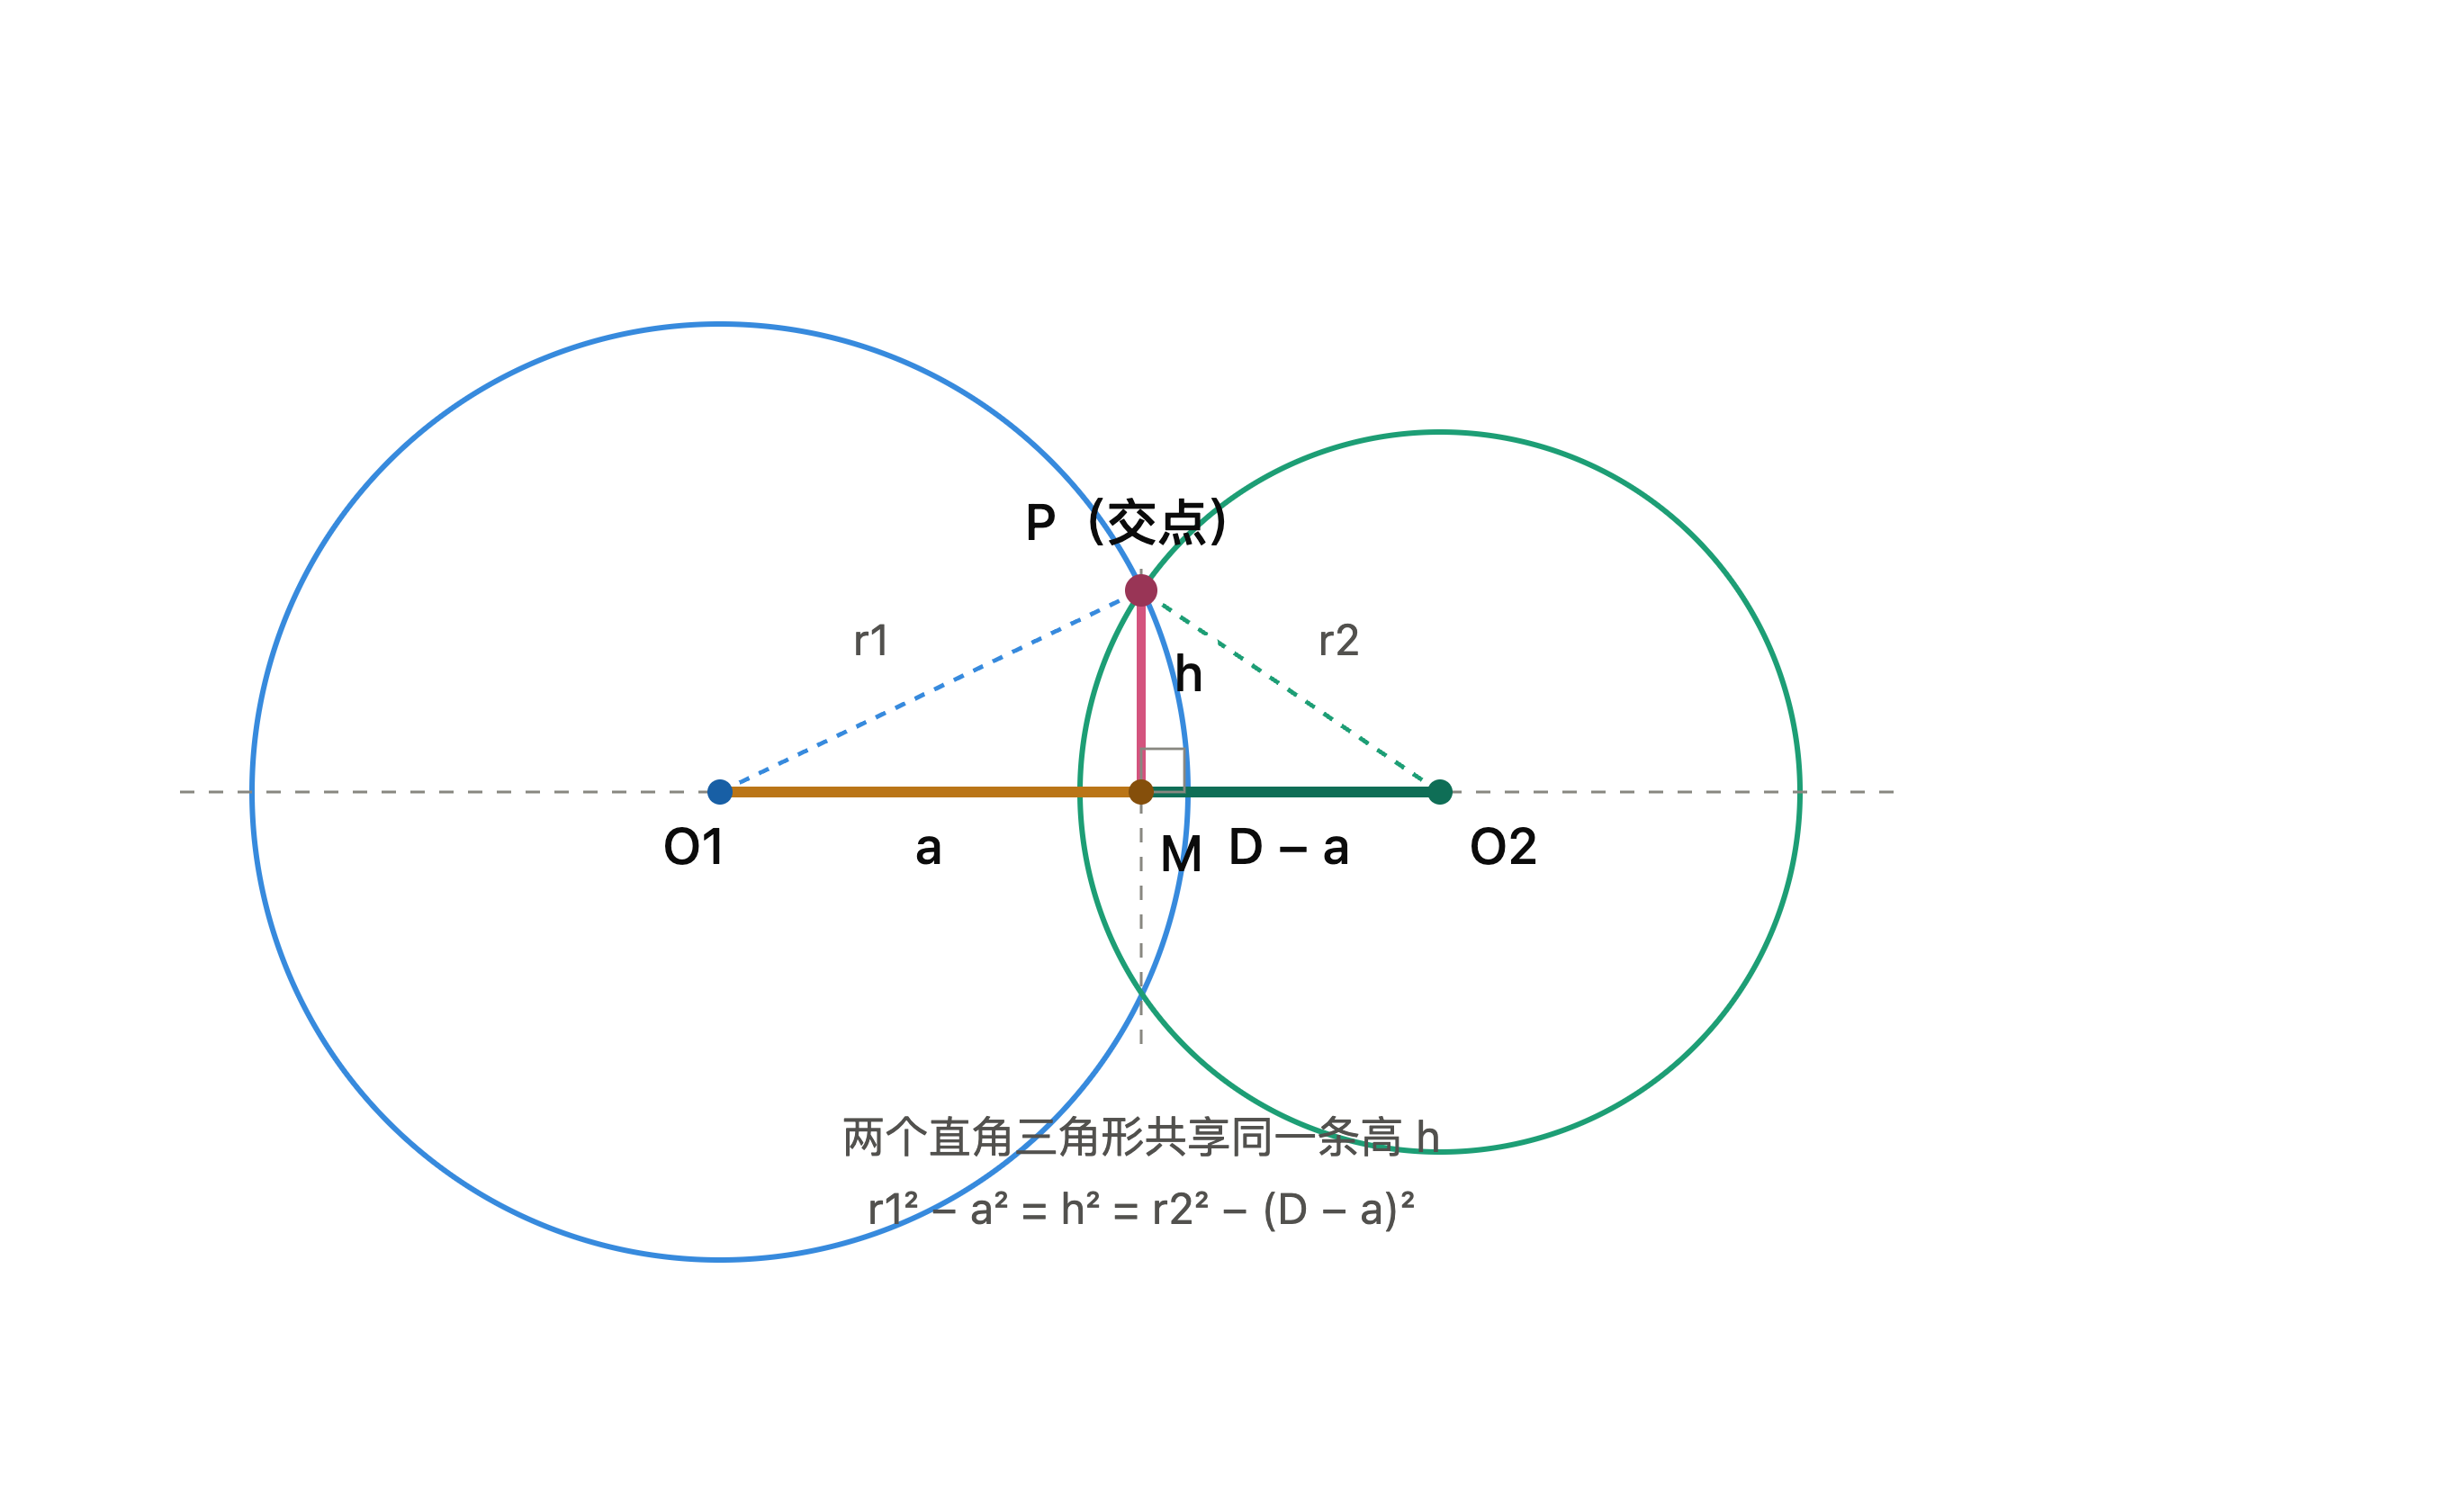
\includegraphics[width=0.88\linewidth]{image/circle_cross_chord_midpoint.png}
		\end{center}

		图中 $PM \perp O_1O_2$ 把 $\triangle O_1PO_2$ 切成两个共享高 $h$ 的直角三角形，两边各写一遍勾股定理就得到 $a$ 的闭式：
		$$
			r_1^2 - a^2 = h^2 = r_2^2 - (D - a)^2
			\;\Longrightarrow\;
			a = \frac{r_1^2 - r_2^2 + D^2}{2D}
		$$
		注意 $a$ \textbf{可以是负数}（$M$ 落在 $O_1$ 背离 $O_2$ 的一侧，两圆一大一小且圆心很近时会出现），公式和代码都不需要特判——$\hat{d} \cdot a$ 自动往反方向走。

		\textbf{重合圆 sentinel}：同心同径时 \texttt{circle\_circle\_relation} 返 $-1$（交点无穷多），\texttt{getCrossPointsCC} 据此返空，重合语义由 caller 自己处理。

		\textbf{类型提示}：标量除法返回公共类型，\texttt{(c2.c - c1.c) / D} 在圆心是 \texttt{Point<ll>}、$D$ 是 \texttt{DB} 时直接得到 \texttt{Point<DB>}，不会截断；代码里先写 \texttt{Point<DB> d = c2.c - c1.c;} 只是为了后面复用 \texttt{d}。

		% geometry-code: circle-circle
\begin{minted}{cpp}
// 依赖：Circle。关系：-1 重合 / 0 不交 / 1 相切 / 2 相交；重合与不交都返回空
template<class T>
int circle_circle_relation(Circle<T> a, Circle<T> b) {
	auto d2 = distancePPNorm(a.c, b.c);
	if (!sgn(d2) && !sgn(a.r - b.r)) return -1;
	int o = sgn(d2 - squared(a.r + b.r)), i = sgn(d2 - squared(a.r - b.r));
	return o > 0 || i < 0 ? 0 : o && i ? 2 : 1;
}
template<class T>
vector<Point<DB>> getCrossPointsCC(Circle<T> c1, Circle<T> c2) {
	int k = circle_circle_relation(c1, c2);
	if (k <= 0) return {};
	Point<DB> d = c2.c - c1.c;
	DB D = d.abs(), a = ((DB)c1.r * c1.r - (DB)c2.r * c2.r + D * D) / (2 * D); // 弦中点到 c1 的有向距离
	Point<DB> m = c1.c + d / D * a;
	if (k == 1) return {m};
	Point<DB> h = d.rot90() / D * (DB)sqrtl(max((DB)0, (DB)c1.r * c1.r - a * a)); // 半弦向量
	return {m + h, m - h};
}
\end{minted}

		\subsection{过一点圆的切点 \texttt{getTangentPoints}}

		\href{https://vjudge.net/solution/69929512}{vjudge 提交}（\href{https://vjudge.net/problem/Aizu-CGL_7_F}{Aizu CGL\_7\_F}）。

		\textbf{推导}：过外部点 $P$ 作圆 $(C, r)$ 切线时，切点 $T$ 同时满足 $PT \perp CT$ 与 $|CT| = r$，即 $\triangle PCT$ 在 $T$ 处是直角三角形，$|PT| = \sqrt{|PC|^2 - r^2}$。切点 $T$ 同时落在原圆 $(C, r)$ 与辅圆 $(P, |PT|)$ 上，对两圆求交即得。

		\textbf{三种退化分类直接 early return}：$P$ 在圆内（含圆心）返空；$P$ 在圆上唯一切点就是 $P$ 自身；$P$ 在圆外才走辅圆链。比"全部喂给 \texttt{getCrossPointsCC} 让它兜底"显式可读，也免依赖辅圆 r = 0 时的边界稳定性。

		% geometry-code: point-tangents
\begin{minted}{cpp}
// 依赖：getCrossPointsCC。圆内无切点，圆上返回自身，圆外与辅圆 (P, |PT|) 求交
vector<Point<DB>> getTangentPoints(Point<ll> P, Circle<ll> cir) {
	i128 d = (P - cir.c).norm() - squared(cir.r);
	if (d < 0) return {};
	if (!d) return {Point<DB>(P)};
	return getCrossPointsCC(Circle<DB>(cir), Circle<DB>(P, sqrtL(d)));
}
\end{minted}

		\subsection{两圆公切线 \texttt{getCommonTangentPoints}}

		\href{https://vjudge.net/solution/69929554}{vjudge 提交}（\href{https://vjudge.net/problem/Aizu-CGL_7_G}{Aizu CGL\_7\_G}）。函数返回的是公切线在 $c_1$ 上的切点列表（每条公切线一个点；对应 $c_2$ 上的切点由切线本身确定）。

		\textbf{推导}：设 $T_1 = c_1.c + r_1 \cdot \vec{n}$，$\vec{n}$ 是单位法向量。令 $\vec{u} = (c_2.c - c_1.c) / D$，分外 / 内公切两类：
		\begin{itemize}
			\setlength\itemsep{0pt}
			\item 外公切：两边法向同向，$T_2 = c_2.c + r_2 \cdot \vec{n}$ 且 $(T_2 - T_1) \perp \vec{n}$，得 $(c_2.c - c_1.c) \cdot \vec{n} = r_1 - r_2$，故 $\cos \alpha = (r_1 - r_2) / D$；
			\item 内公切：两边法向反向，$T_2 = c_2.c - r_2 \cdot \vec{n}$，得 $\cos \alpha = (r_1 + r_2) / D$。
		\end{itemize}
		然后 $\vec{n} = \cos \alpha \cdot \vec{u} + \sin \alpha \cdot \vec{u}_\perp$，$\sin \alpha = \pm \sqrt{1 - \cos^2 \alpha}$ 取两组。

		\textbf{退化}：$|\cos \alpha| > 1$ 该类无切（内含 / 包含跳过）；$\sin \alpha = 0$ 该类只 1 条（内 / 外切临界）；$D = 0$（同心，含重合）统一返空。最后 \texttt{sort + unique} 去重，应对内 / 外切临界 + $r = 0$ 退化下 4 个候选近重合的情形。

		% geometry-code: common-tangents
\begin{minted}{cpp}
// 依赖：Circle。返回各公切线在 c1 上的切点（外公切 + 内公切，已去重）；同心（含重合）返回空
vector<Point<DB>> getCommonTangentPoints(Circle<ll> c1, Circle<ll> c2) {
	vector<Point<DB>> ret;
	Point<DB> d = c2.c - c1.c;
	DB D = d.abs(), r1 = c1.r, r2 = c2.r;
	if (D < eps) return ret;
	for (DB cs : {(r1 - r2) / D, (r1 + r2) / D}) { // 法向与连心线夹角的 cos：外公切 / 内公切
		if (cs > 1 + eps || cs < -1 - eps) continue;
		DB sn = sqrtl(max((DB)0, 1 - cs * cs));
		Point<DB> p = c1.c + d / D * (cs * r1), v = d.rot90() / D * (sn * r1);
		ret.push_back(p + v);
		if (sn >= eps) ret.push_back(p - v);
	}
	sort(ret.begin(), ret.end());
	ret.erase(unique(ret.begin(), ret.end()), ret.end());
	return ret;
}
\end{minted}

		\subsection{两圆交集面积 \texttt{two\_circle\_intersect\_area}}

		\href{https://vjudge.net/solution/69929585}{vjudge 提交}（\href{https://vjudge.net/problem/Aizu-CGL_7_I}{Aizu CGL\_7\_I}）。

		\textbf{推导}：两圆相交时公共弦把每个圆切成两个弓形（segment / cap）。交集面积 = $c_1$ 靠 $c_2$ 那侧的弓形 + $c_2$ 靠 $c_1$ 那侧的弓形。圆心角由余弦定理给出：
		$$\theta_1 = 2 \arccos \frac{D^2 + r_1^2 - r_2^2}{2 D r_1}, \quad \theta_2 = 2 \arccos \frac{D^2 + r_2^2 - r_1^2}{2 D r_2}.$$
		单个弓形面积 $= \tfrac{1}{2} r^2 (\theta - \sin \theta)$。

		\textbf{边界}：$D \ge r_1 + r_2$ 不交 $\to 0$；$D \le |r_1 - r_2|$ 一圆完全包含另一圆 $\to \pi \cdot r_{\min}^2$（重合圆自然落入此档，无需特判）。

		% geometry-code: circle-area
\begin{minted}{cpp}
// 依赖：Circle, distancePP。相交时 = 两个弓形之和
template<class T>
DB two_circle_intersect_area(Circle<T> c1, Circle<T> c2) {
	DB D = distancePP(c1.c, c2.c), r1 = c1.r, r2 = c2.r;
	if (sgn(D - r1 - r2) >= 0) return 0;
	if (sgn(D - fabsl(r1 - r2)) <= 0) return PI * min(r1, r2) * min(r1, r2);
	auto seg = [&](DB r, DB o) { // 圆 r 上、靠向圆 o 的弓形
		DB t = 2 * acosl(clamp((D * D + r * r - o * o) / (2 * D * r), (DB)-1, (DB)1));
		return r * r * (t - sinl(t)) / 2;
	};
	return seg(r1, r2) + seg(r2, r1);
}
\end{minted}

		\subsection{简单多边形与圆的交集面积 \texttt{polygon\_circle\_intersect\_area}}

		\href{https://vjudge.net/solution/69929628}{vjudge 提交}（\href{https://vjudge.net/problem/Aizu-CGL_7_H}{Aizu CGL\_7\_H}）。

		\textbf{核心}：把多边形按边累加「三角形 $(O, A_i, A_{i+1})$ 与 disk $(O, r)$ 的有向面积」，$O$ 是圆心。每条边的贡献由 \texttt{tri\_disk\_signed\_area} 计算：先把 $A, B$ 平移到以 $O$ 为原点的坐标系；统一求边在圆内的参数区间，并截到 $[0,1]$。区间两侧算扇形，中间算三角形；这同时覆盖以下四种情况：
		\begin{itemize}
			\setlength\itemsep{0pt}
			\item 两端都在圆内：整段就是真三角形，有向面积 $= \tfrac{1}{2} \mathrm{cross}(A, B)$；
			\item 两端都在圆外但弦穿圆得入 / 出两点 $P_1, P_2$：扇形 $OAP_1$ + 真三角形 $OP_1 P_2$ + 扇形 $OP_2 B$；
			\item 两端都在圆外且不穿圆：整段对应一个扇形（从 $\vec{OA}$ 转到 $\vec{OB}$）；
			\item $A$ 内 $B$ 外（或反之）：在边上找穿圆点 $P$，$OAP$ 是真三角形 + $OPB$ 是扇形。
		\end{itemize}
		最后整圈累加取 \texttt{abs}，输入多边形 CW / CCW 都可。\textbf{扇形角度用 \texttt{atan2(cross, dot)} 算}：能拿到有向角度 $\in (-\pi, \pi]$，正负自动包含弧的方向（不像 \texttt{acos} 只给 $[0, \pi]$ 丢方向信息）。

		\textbf{退化}：\texttt{tri\_disk\_signed\_area} 在 $A = B$（多边形相邻顶点重合）时直接返 0，整体也吃得到。

		% geometry-code: polygon-circle
\begin{minted}{cpp}
// 依赖：Circle。三角形 (O, A, B) 与圆盘 (O, r) 的有向交面积，A、B 已平移到以圆心 O 为原点
DB tri_disk_signed_area(Point<DB> A, Point<DB> B, DB r) {
	if (A == B) return 0;
	auto sector = [&](Point<DB> p, Point<DB> q) { return r * r * atan2l(cross(p, q), dot(p, q)) / 2; };
	Point<DB> d = B - A;
	DB dd = d.norm(), ad = dot(A, d), disc = ad * ad - dd * (A.norm() - r * r);
	if (disc <= 0) return sector(A, B);
	DB s = sqrtl(disc), l = max((DB)0, (-ad - s) / dd), h = min((DB)1, (-ad + s) / dd); // 边在圆内的参数区间
	if (l >= h) return sector(A, B);
	Point<DB> P = A + d * l, Q = A + d * h;
	return sector(A, P) + cross(P, Q) / 2 + sector(Q, B);
}
// 简单多边形（CW / CCW 均可）与圆的交集面积
template<class T>
DB polygon_circle_intersect_area(Circle<DB> cir, const vector<Point<T>> &poly) {
	DB res = 0;
	int n = poly.size();
	for (int i = 0; i < n; ++i) res += tri_disk_signed_area(poly[i] - cir.c, poly[(i + 1) % n] - cir.c, cir.r);
	return res < 0 ? -res : res;
}
\end{minted}

		\subsection{多边形凸性检验}

		\textbf{允许的输入}：\textcolor{red}{\textbf{不允许自交}}的多边形，顺序可顺可逆，函数会顺手把 \texttt{poly} 旋转 / 反向到「最左下点位 \texttt{[0]} + CCW 顺序」。

		下面是三类\textbf{不被认为是凸多边形}的反例。

		\subsubsection{反例 1：内角为反向凹角（外角为锐角）}

		外角是锐角时 $\sin > 0$，叉乘也 $> 0$，看似 CCW；但其实形成的是\textcolor{red}{凹陷}。

		\begin{center}
			\begin{tikzpicture}[>=Stealth]
				\draw[thick] (0,0) -- (3,0) -- (3,2) -- (1.5,1) -- (0,2) -- cycle;
				\fill[red] (1.5,1) circle (2pt);
				\node[font=\scriptsize, color=red, anchor=west] at (1.6,1) {反向凹角};
			\end{tikzpicture}

			\vspace{2pt}
			{\footnotesize\sffamily\color{gray} 图注：标红顶点的内角 $> 180^{\circ}$（反射角），\texttt{isConvex} 中相对 \texttt{poly[0]} 的扇形检查 \texttt{cross(poly[0], poly[i], poly[i+1]) < strict} 触发返回 false。}
		\end{center}

		\subsubsection{反例 2：自交多边形（蝴蝶结）}

		\begin{center}
			\begin{tikzpicture}[>=Stealth]
				\draw[thick] (0,0) -- (3,2) -- (3,0) -- (0,2) -- cycle;
				\fill[red] (1.5,1) circle (2pt);
				\node[font=\scriptsize, color=red, anchor=west] at (1.6,1) {自交点};
			\end{tikzpicture}

			\vspace{2pt}
			{\footnotesize\sffamily\color{gray} 图注：四个顶点排成蝴蝶结，相对 \texttt{poly[0]} 不再是单调 CCW 排列，扇形检查即被排除。}
		\end{center}

		\subsubsection{反例 3：内角恰为 $180^{\circ}$}

		三点共线（叉乘 \texttt{= 0}）也不允许，否则会让边数虚假增加。

		\begin{center}
			\begin{tikzpicture}[>=Stealth]
				\draw[thick] (0,0) -- (1.5,0) -- (3,0) -- (1.5,2.2) -- cycle;
				\fill[red] (1.5,0) circle (2pt);
				\node[font=\scriptsize, color=red, anchor=north] at (1.5,-0.05) {$180^{\circ}$};
			\end{tikzpicture}

			\vspace{2pt}
			{\footnotesize\sffamily\color{gray} 图注：底边上多了一个 $180^{\circ}$ 顶点，相邻两边叉乘 \texttt{s < strict} 在 \texttt{s = 0} 时触发返回 false（严格模式要求大于零）。}
		\end{center}

		\textbf{实现}：\texttt{reorder\_polygon} 把多边形旋转 / 反向到「最左下点位 \texttt{[0]} + CCW 顺序」，再在同一个循环里检查两件事：(a)~每个内角（相邻两边的叉乘）符号合规；(b)~所有顶点相对于 \texttt{poly[0]} 按 CCW 排列。

		\textbf{\texttt{reorder\_polygon} 用整体 \texttt{polygonSignedArea} 判方向}，\textcolor{red}{\textbf{不要}}用「前三点 \texttt{cross}」局部判向：含三点共线的多边形（如长方形 + 边密集共线）前三点 \texttt{cross = 0}，会被旧版 \texttt{<= 0} 误判为 CW 而强 reverse，下游 \texttt{isConvex} / 旋转卡壳全部失效（QOJ 784 实测）。

		\textbf{\texttt{isConvex} 加 \texttt{strict} 参数}：
		\begin{itemize}
					\setlength\itemsep{0pt}
				\item \texttt{strict = true}（默认）：严格凸，拒绝三点共线 / 内角 = $180^{\circ}$；
				\item \texttt{strict = false}：弱凸，允许内角 = $180^{\circ}$（题面用「凸」时常允许共线，要的就是这个口径）。
		\end{itemize}
		\textbf{加宽接受范围有时是发现底层 bug 的好工具}：本次就是因为加 \texttt{strict = false} 后 lax 模式 fail，才暴露出 \texttt{reorder\_polygon} 的隐藏 bug——strict 模式因为 \texttt{<= 0} 提前 short-circuit 把它掩盖了。

		% geometry-code: reorder
\begin{minted}{cpp}
// 依赖：polygonSignedArea。整理成 CCW 且 [0] 为 y 最小（再 x 最小）的点；整体面积判向，不受前三点共线影响
template<class T>
void reorder_polygon(vector<Point<T>> &poly) {
	if (sgn(polygonSignedArea(poly)) < 0) reverse(poly.begin(), poly.end());
	auto byY = [](Point<T> a, Point<T> b) { return tie(a.y, a.x) < tie(b.y, b.x); };
	rotate(poly.begin(), min_element(poly.begin(), poly.end(), byY), poly.end());
}
\end{minted}

% geometry-code: is-convex
\begin{minted}{cpp}
// 依赖：reorder_polygon。不允许自交，顺序任意（会整理成 CCW）。strict：拒绝内角 180°（三点共线）
// AC https://qoj.ac/submission/2002121
template<class T>
bool isConvex(vector<Point<T>> poly, bool strict = true) {
	int n = poly.size();
	if (n <= 2) return false;
	reorder_polygon(poly);
	bool turn = false; // 至少一处真左转，排除全共线
	for (int i = 0; i < n; ++i) {
		int s = sgn(cross(poly[i], poly[(i + 1) % n], poly[(i + 2) % n]));
		if (s < strict) return false;
		turn |= s > 0;
		// 所有顶点相对 poly[0] 也要按 CCW 排列，否则是星形 / 乱序
		if (i && i < n - 1 && sgn(cross(poly[0], poly[i], poly[i + 1])) < strict) return false;
	}
	return turn;
}
\end{minted}

		\subsection{点与多边形关系}

		多边形未必凸——「有向面积一定为正」的方法在凹多边形上失效，所以采用经典的\textbf{射线奇偶法}。

		\begin{center}
			\begin{tikzpicture}[>=Stealth]
				\draw[thick] (0,0) -- (3.2,0.3) -- (3.6,2) -- (2.2,1.4) -- (2,2.7) -- (0.5,2.2) -- cycle;
				\coordinate (Pin)  at (1.4, 1.4);
				\coordinate (Pout) at (1.4, -0.6);
				\fill[red]   (Pin)  circle (2pt) node[above, font=\scriptsize, color=red]   {$P_{\text{in}}$};
				\fill[blue]  (Pout) circle (2pt) node[below, font=\scriptsize, color=blue]  {$P_{\text{out}}$};
				\draw[->, dashed, red]  (Pin)  -- (5.0, 1.4);
				\draw[->, dashed, blue] (Pout) -- (5.0, -0.6);
				\node[font=\tiny, color=red,  anchor=south] at (4.0, 1.45) {1 次相交（奇）→ 在内};
				\node[font=\tiny, color=blue, anchor=north] at (4.0, -0.65) {0 次相交（偶）→ 在外};
			\end{tikzpicture}

			\vspace{2pt}
			{\footnotesize\sffamily\color{gray} 图注：从待判定点向任意方向打一条射线，统计与多边形边的相交次数。\textbf{奇 = 在内，偶 = 在外}。代码使用水平射线，边的纵坐标采用半开区间 $[y_{\min},y_{\max})$，穿过顶点时只计一次。}
		\end{center}

		返回值约定：\texttt{2}~=~严格在内、\texttt{1}~=~点落在某条边上、\texttt{0}~=~严格在外。

		% geometry-code: point-in-polygon
\begin{minted}{cpp}
// 依赖：CCW。水平射线 + 半开区间计数：0 外部 / 1 边界 / 2 内部；凹多边形也可
template<class T>
int isInPolygon(Point<T> p, const vector<Point<T>> &poly) {
	bool inside = false;
	int n = poly.size();
	for (int i = 0; i < n; ++i) {
		auto a = poly[i], b = poly[(i + 1) % n];
		if (CCW(p, Line<T>(a, b)) == ON_SEGMENT) return 1;
		if (a.y > b.y) swap(a, b);
		if (a.y <= p.y && p.y < b.y && cross(a, b, p) > 0) inside = !inside;
	}
	return inside ? 2 : 0;
}
\end{minted}

		\subsection{极角排序}

		按 \texttt{atan2(y, x)} 排序时，注意 \texttt{atan2} 浮点本身的精度问题。\textbf{规避调用 atan2} 的做法：先按「下半平面 / x 轴正向 / 上半平面」三档分桶，桶内再用叉乘符号判定相对方位。这样所有比较都用整数叉乘完成，没有浮点误差。

		起点是 $x$ 轴正半轴（含原点），逆时针环绕一周到 $x$ 轴负半轴（不含）。

		% geometry-code: polar-sort
\begin{minted}{cpp}
// 依赖：点线基础。极角序：x 正半轴（含原点）起逆时针一圈；全整数叉积，不用 atan2
template<class T>
int get_part_of_point(Point<T> p) { return p.y < 0 ? 0 : p.y == 0 && p.x >= 0 ? 1 : 2; }
template<class T> // AC https://qoj.ac/submission/2001485
void polar_angle_sort(vector<Point<T>> &a) {
	sort(a.begin(), a.end(), [](Point<T> p, Point<T> q) {
		int u = get_part_of_point(p), v = get_part_of_point(q);
		return u != v ? u < v : cross(p, q) > 0;
	});
}
// 有向直线按方向向量极角排序；同向的线「左半平面更紧」的排前（半平面交用）
template<class T>
void polar_angle_sort(vector<Line<T>> &a) {
	sort(a.begin(), a.end(), [](Line<T> l, Line<T> m) {
		Point<T> p = l.p2 - l.p1, q = m.p2 - m.p1;
		int u = get_part_of_point(p), v = get_part_of_point(q);
		if (u != v) return u < v;
		if (auto c = cross(p, q)) return c > 0;
		return cross(p, m.p1 - l.p1) < 0;
	});
}
// 排序后同向线只留每组最紧的一条（即每组第一条）
template<class T>
void unique_line_polar_angle_sort(vector<Line<T>> &a) {
	polar_angle_sort(a);
	a.erase(unique(a.begin(), a.end(), [](Line<T> l, Line<T> m) {
		Point<T> p = l.p2 - l.p1, q = m.p2 - m.p1;
		return get_part_of_point(p) == get_part_of_point(q) && cross(p, q) == 0;
	}), a.end());
}
\end{minted}

		\subsection{Minkowski 闵可夫斯基和}

		给定两个凸包 $P_1$、$P_2$，定义其闵可夫斯基和：
		$$
		P_1 \oplus P_2 = \{a + b \mid a \in P_1,\ b \in P_2\}
		$$
		结果仍是凸包。\textbf{减法}就等价于「加上对方关于原点的中心对称图形」，这是判断两凸包是否相交、求最近距离的常用技巧。

		\begin{center}
			\begin{tikzpicture}[>=Stealth]
				\begin{scope}
					\draw[blue, thick] (-0.6,-0.6) rectangle (0.6, 0.6);
					\node[font=\scriptsize] at (0, -1.0) {$P_1$};
				\end{scope}
				\begin{scope}[xshift=2.0cm]
					\node[font=\scriptsize, anchor=center] at (-0.85, 0) {$\oplus$};
					\draw[orange, thick] (0,0) circle (0.4);
					\node[font=\scriptsize] at (0, -1.0) {$P_2$};
				\end{scope}
				\begin{scope}[xshift=4.4cm]
					\node[font=\scriptsize, anchor=center] at (-0.95, 0) {$=$};
					\draw[teal, thick] (-0.6, -1.0) -- (0.6, -1.0);
					\draw[teal, thick] (-0.6,  1.0) -- (0.6,  1.0);
					\draw[teal, thick] (-1.0, -0.6) -- (-1.0, 0.6);
					\draw[teal, thick] ( 1.0, -0.6) -- (1.0,  0.6);
					\draw[teal, thick] (0.6, 1.0)  arc (90:0:0.4);
					\draw[teal, thick] (1.0, -0.6) arc (0:-90:0.4);
					\draw[teal, thick] (-0.6, -1.0) arc (270:180:0.4);
					\draw[teal, thick] (-1.0, 0.6)  arc (180:90:0.4);
					\node[font=\scriptsize] at (0, -1.4) {$P_1 \oplus P_2$};
				\end{scope}
			\end{tikzpicture}

			\vspace{2pt}
			{\footnotesize\sffamily\color{gray} 图注：正方形 + 圆 = 圆角矩形——四条直边长度等于原正方形的边长，四个角是半径等于圆半径的四分之一圆弧（这是几何上严格的 Minkowski 和）。}
		\end{center}

		\textbf{算法核心}：先把两个凸包都 \texttt{reorder\_polygon}（最左下点起、CCW 顺序），然后\textbf{把它们的边向量按极角合并}（类似归并排序的归并步）：每次比较两条候选边向量的叉乘符号，挑极角更小的那条接到答案末尾。起点设为 $P_1[0] + P_2[0]$，沿合并后的边向量逐条累加即得新凸包。

		% geometry-code: minkowski
\begin{minted}{cpp}
// 依赖：reorder_polygon。输入凸多边形（可退化为点 / 线段），原地整理；返回闭合边界（末点重复首点），保留共线边
template<class T>
vector<Point<T>> minkowski(vector<Point<T>> &P1, vector<Point<T>> &P2) {
	if (P1.empty() || P2.empty()) return {};
	reorder_polygon(P1); reorder_polygon(P2);
	int n = P1.size(), m = P2.size(), i = 0, j = 0;
	vector<Point<T>> ans{P1[0] + P2[0]};
	while (i < n || j < m) { // 按极角归并两组边向量
		auto a = P1[(i + 1) % n] - P1[i % n], b = P2[(j + 1) % m] - P2[j % m];
		bool takeA = j == m || (i < n && cross(a, b) > 0);
		ans.push_back(ans.back() + (takeA ? a : b));
		takeA ? ++i : ++j;
	}
	return ans;
}
\end{minted}

		\subsection{半平面交（half\_plane\_cut）}

		把每条有向直线 \texttt{Line(p1, p2)} 看作半平面 ——「沿 \texttt{p1 → p2} 方向走，左手边」是合法区域。所有半平面的交集若非空则为一个凸多边形（可能退化为无界、零面积等情形，本模板返回 \texttt{vector<Point<DB>>}，空表示交集为空 / 退化）。

		\textbf{算法核心}：双端队列扫描法。先 \texttt{unique\_line\_polar\_angle\_sort} 把直线按极角排序 + 同向去重，然后逐条加入 deque \texttt{q}：每次新直线 \texttt{l} 进来，先用 \texttt{l} 反向清理队尾（队尾两条线的交点若在 \texttt{l} 右侧，说明该交点被 \texttt{l} 切掉，对应的队尾线已经无贡献），再清理队首（对称地）；扫完一轮后还要做一次 \textbf{wrap-around}：用队首 / 队尾互相再清一遍（处理环形闭合时残留的失效线段）。

		\textbf{复杂度}：$O(N \log N)$（瓶颈是极角排序，扫描本身均摊 $O(N)$）。

		\textbf{常见用法}：
		\begin{itemize}
			\item \textbf{多个半平面求公共凸区域}：每个不等式 $a_i x + b_i y \le c_i$ 表示一个半平面，加入对应的有向直线即可。
			\item \textbf{多边形并的总面积（旋转切割型）}：经典题 \href{https://vjudge.net/problem/OpenJ_Bailian-2451}{\emph{Uyuw's Concert}}（多次直线切凸多边形求剩余面积）/ \href{https://www.luogu.com.cn/problem/P4196}{洛谷 P4196 [CQOI2006] 凸多边形}（多个凸多边形求交）。
			\item \textbf{有界化}：当输入只有半平面、没有边界 box 时，可手动加 4 条「大正方形边界」直线（如 \texttt{[-1e9, 1e9]} 见方），避免交集无界。
		\end{itemize}

		% geometry-code: half-planes
\begin{minted}{cpp}
// 依赖：unique_line_polar_angle_sort, getintersect。p1 -> p2 左侧闭半平面；求有界、正面积交集，
// 空 / 无界 / 退化返回空。无界输入需自行加题目允许的边界
template<class T>
vector<Point<DB>> half_plane_cut(vector<Line<T>> lines) {
	unique_line_polar_angle_sort(lines);
	deque<Line<T>> q;
	auto out = [&](Line<T> a, Line<T> b, Line<T> c) { return sgn(cross(c.p1, c.p2, getintersect(a, b))) < 0; };
	auto para = [&](Line<T> a, Line<T> b) { return cross(a.p2 - a.p1, b.p2 - b.p1) == 0; };
	for (auto l : lines) {
		while (q.size() > 1 && out(q[q.size() - 2], q.back(), l)) q.pop_back();
		while (q.size() > 1 && out(q[0], q[1], l)) q.pop_front();
		if (!q.empty() && para(q.back(), l)) return {}; // 反向平行：交集为空或退化
		q.push_back(l);
	}
	while (q.size() > 2 && out(q[q.size() - 2], q.back(), q.front())) q.pop_back();
	while (q.size() > 2 && out(q[0], q[1], q.back())) q.pop_front();
	if (q.size() < 3) return {};
	vector<Point<DB>> poly;
	for (int i = 0; i < (int)q.size(); ++i) {
		if (para(q[i], q[(i + 1) % q.size()])) return {};
		poly.push_back(getintersect(q[i], q[(i + 1) % q.size()]));
	}
	return poly;
}
\end{minted}

		\textbf{使用范例}（Uyuw's Concert 框架：给定 $N$ 条有向直线 + 题目自带的 $[0, 10000]^2$ 边界，求公共半平面交的面积）：

		\begin{minted}{cpp}
ll N; cin >> N;
vector<Line<DB>> lines(N);
for (auto &l : lines) cin >> l;
// 手动补 4 条边界直线（CCW 顺序：左下→右下→右上→左上）
auto a1 = Point<DB>(0, 0), a2 = Point<DB>(10000, 0);
auto a3 = Point<DB>(10000, 10000), a4 = Point<DB>(0, 10000);
lines.push_back(Line<DB>(a1, a2));
lines.push_back(Line<DB>(a2, a3));
lines.push_back(Line<DB>(a3, a4));
lines.push_back(Line<DB>(a4, a1));
auto poly = half_plane_cut(lines);
cout << fsp(1) << polygonArea(poly) << "\n";
		\end{minted}

		\subsection{凸包（Andrew 算法）}

		按 $x$ 升序、$x$ 相同按 $y$ 升序排序后，从左到右扫一遍维护下凸包，再从右到左扫一遍维护上凸包，把两段拼起来即可。

		\textbf{\texttt{strict} 参数}决定共线点处理：\texttt{strict = true} 时 \texttt{cross == 0}（共线）也弹栈，\textbf{不保留共线点}；\texttt{strict = false} 时只在 \texttt{cross < 0}（凹陷）才弹，\textbf{保留共线点}（题目要求「凸包上所有点」时用）。

		\textbf{\texttt{HullMode} 参数}：三种返回都是 CCW 方向。\texttt{HULL\_FULL} 完整凸包（\textbf{按 $Y$ 排序}，从\textbf{最低点}（$y$ 最小、再 $x$ 最小）起 CCW 绕一圈；这样剥层第一步就拿到最低点起步，不必再调 \texttt{reorder\_polygon} 找最低点）；\texttt{HULL\_LOWER} 下凸壳（最左 $\to$ 最右）；\texttt{HULL\_UPPER} 上凸壳（最右 $\to$ 最左，复用单调栈函数反向扫描）。\textbf{易踩}：\texttt{HULL\_UPPER} 等价「直线上半包络」时调用前需 dedupe 同斜率（strict 处理不了「同 $x$ 不同 $y$ 竖边」退化），见 STL 节 \texttt{sort + unique} 模板。

		% geometry-code: convex-hull
\begin{minted}{cpp}
// 依赖：polygonSignedArea。strict：不保留共线点。FULL 从最低点起 CCW；LOWER 左到右；UPPER 右到左
enum HullMode { HULL_FULL, HULL_LOWER, HULL_UPPER };
template<class T>
vector<Point<T>> make_convex_hull(vector<Point<T>> A, bool strict, HullMode mode) {
	if (mode == HULL_FULL) sort(A.begin(), A.end(), [](Point<T> a, Point<T> b) { return tie(a.y, a.x) < tie(b.y, b.x); });
	else sort(A.begin(), A.end());
	A.erase(unique(A.begin(), A.end()), A.end());
	int n = A.size();
	if (n <= 2) {
		if (mode == HULL_UPPER) reverse(A.begin(), A.end());
		return A;
	}
	auto chain = [&](int start, int step) { // 单调栈扫一侧
		vector<Point<T>> h;
		for (int i = start; i >= 0 && i < n; i += step) {
			while (h.size() > 1 && sgn(cross(h[h.size() - 2], h.back(), A[i])) < strict) h.pop_back();
			h.push_back(A[i]);
		}
		return h;
	};
	if (mode == HULL_LOWER) return chain(0, 1);
	if (mode == HULL_UPPER) return chain(n - 1, -1);
	auto h = chain(0, 1), u = chain(n - 1, -1);
	h.pop_back(); u.pop_back();
	h.insert(h.end(), u.begin(), u.end());
	return !strict && !sgn(polygonSignedArea(h)) ? A : h; // 全共线且保留共线点：直接返回排好序的点
}
\end{minted}

		\subsubsection{对偶点技巧：直线上半包络 $\Leftrightarrow$ 对偶点上凸壳}

		\href{https://www.luogu.com.cn/problem/P3194}{洛谷 P3194 [HNOI2008] 水平可见直线}：给 $N$ 条直线 $y = A_i x + B_i$，从 $y = +\infty$ 俯视，问哪些「有某段 $x$ 露头」。

		\textcolor{blue}{\textbf{直线-点对偶}}：把 $L_i$ 映射到对偶平面的点 $P_i = (A_i, B_i)$，则
		\[
			L_i \text{ 可见} \iff P_i \text{ 在所有对偶点的「严格上凸壳」上.}
		\]
		\textbf{为什么}：3 条 $a_1 < a_2 < a_3$，$L_2$ 被 $L_1, L_3$ 在某 $x$ 处压下 $\iff \mathrm{cross}(P_2 - P_1,\, P_3 - P_1) \ge 0$（$P_2$ 在 $P_1 P_3$ 下方或共线）。共线时三线共点、$L_2$ 只在一点露头不是 segment，\texttt{strict} 模式正好弹掉。

		\begin{center}
			\begin{tikzpicture}[>=Stealth, font=\scriptsize]
				% ===== Primal plane =====
				\begin{scope}[x=0.55cm, y=0.45cm]
					\draw[->, gray] (-1.7, 0) -- (1.9, 0) node[right] {$x$};
					\draw[->, gray] (0, -1.3) -- (0, 3.6) node[left] {$y$};
					% 4 条线全画（细灰）
					\draw[blue!25, thin] (-1.5,  4)   -- (1.5, -2);   % L1: y = -2x + 1
					\draw[blue!25, thin] (-1.5,  2)   -- (1.5,  2);   % L2: y = 2
					\draw[blue!25, thin] (-1.5, -2)   -- (1.5,  4);   % L4: y = 2x + 1
					% 上半包络（粗蓝）：L1 → 转折(-0.5, 2) → L2 → 转折(0.5, 2) → L4
					\draw[blue, very thick] (-1.5, 4) -- (-0.5, 2) -- (0.5, 2) -- (1.5, 4);
					% L3 被压（灰虚）
					\draw[gray!70, dashed, thin] (-1.5, 2.5) -- (1.5, -0.5);
					% 标签
					\node[blue!70!black, font=\tiny] at (-1.55, 3.55) {$L_1$};
					\node[blue!70!black, font=\tiny] at ( 1.55, 3.55) {$L_4$};
					\node[blue!70!black, font=\tiny] at ( 1.55, 2.35) {$L_2$};
					\node[gray, font=\tiny]          at ( 1.65, -0.7) {$L_3$};
					\node[font=\footnotesize, anchor=south] at (0, 3.8) {\textbf{Primal}};
				\end{scope}

				% ===== Dual plane =====
				\begin{scope}[xshift=4.6cm, x=0.55cm, y=0.7cm]
					\draw[->, gray] (-2.7, 0) -- (2.9, 0) node[right] {$A$};
					\draw[->, gray] (0, -0.4) -- (0, 2.7) node[left] {$B$};
					% 上凸壳（粗蓝）
					\draw[blue, very thick] (-2, 1) -- (0, 2) -- (2, 1);
					% 提示 P3 严格在弦下方的垂直差
					\draw[red!60, dashed, thin] (-1, 1) -- (-1, 1.5);
					% 4 个点
					\fill[blue] (-2, 1) circle (2pt) node[below left,  font=\tiny, color=blue] {$P_1$};
					\fill[blue] ( 0, 2) circle (2pt) node[above,       font=\tiny, color=blue] {$P_2$};
					\fill[blue] ( 2, 1) circle (2pt) node[below right, font=\tiny, color=blue] {$P_4$};
					% P3 被弹（红叉）
					\fill[gray] (-1, 1) circle (1.8pt);
					\draw[red, thick] (-1.18, 0.82) -- (-0.82, 1.18);
					\draw[red, thick] (-1.18, 1.18) -- (-0.82, 0.82);
					\node[gray, font=\tiny, anchor=north] at (-1, 0.85) {$P_3$};
					\node[font=\footnotesize, anchor=south] at (0, 2.85) {\textbf{Dual}};
				\end{scope}
			\end{tikzpicture}

			\vspace{2pt}
			{\footnotesize\sffamily\color{gray} 图注：左 Primal 4 条线，上半包络 = $L_1 \to L_2 \to L_4$（粗蓝折线），$L_3$ 全程在下被压（灰虚线）。右 Dual 4 个对偶点，$P_3 = (-1, 1)$ 严格落在弦 $P_1 P_2$ 下方（红虚示意垂直差 0.5），上凸壳 $P_1 \to P_2 \to P_4$ 不收 $P_3$。\textbf{这就是「$L_i$ 可见 $\Leftrightarrow$ $P_i$ 在上凸壳上」的视觉对照}。}
		\end{center}

		\textbf{落地}：(1) 把 $(A_i, B_i)$ 当点（套 \texttt{Point<ll>} 的 \texttt{id} 字段绑原始下标）；(2) 同 $A$ 多条只留 $B$ 最大那条（\texttt{sort + unique} 模板见 STL 节）；(3) \texttt{make\_convex\_hull(pts, true, HULL\_UPPER)} 直接返回上凸壳点列，按 \texttt{id} 升序输出。$|A|, |B| \le 5 \times 10^5$ 时全程整数，\texttt{cross} 走 \texttt{\_\_int128}。

		\subsection{凸多边形直径（旋转卡壳）}

		\href{https://vjudge.net/problem/QOJ-784}{QOJ 784}（凸多边形直径模板题）。

		给一个 \textbf{逆时针顺序}的 $n$ 凸多边形（允许三点共线），求最远点对的距离。\textcolor{blue}{\textbf{旋转卡壳}}的标准技巧：把每条边 $A[r] \to A[r{+}1]$ 当成一条「卡尺」，对踵点 $A[l]$ 是离这条边最远的顶点。$r$ 沿 CCW 扫一圈时 $l$ 单调（不回退），整体 $O(n)$。

		\textbf{关键判据}：$l$ 该不该往前推一步？看「以边 $(r,\,r{+}1)$ 为底、$l{+}1$ vs $l$ 为顶」的两个三角形面积——后者 $\ge$ 前者就推。\textbf{比直接比距离平方更鲁棒}：曲率非均匀的凸包（如 spike 形 $r(\theta) = 1 + 0.1\sin(7\theta)$）下 $|A[l] - A[r]|^2$ 沿 $r$ 不是单峰会卡死，但「以边为底的三角形面积」仍是单峰。

		\textbf{4 个不要踩的坑}（QOJ 784 session 实录，每个都有真实反例）：
		\begin{enumerate}
					\setlength\itemsep{0pt}
				\item \textbf{不要做点对踵}：以 $|A[l] - A[r]|^2$ 沿 $r$ 找单峰只在「曲率均匀」凸包成立，cyaron 默认凸包形是盲区——必死于 spike 形；
				\item \textbf{$l, r$ 角色不能反}：必须「外层 $r$ 是边、内层 $l$ 是点」，反过来 $|\text{edge}|$ 乘子会破坏单峰；
				\item \textbf{ans 候选取两个}：$(A[l], A[r])$ 和 $(A[l], A[r{+}1])$ 都要更新，只取一个会漏掉「边端点本身就是最远对」的情形；
				\item \textbf{推进用 $\le$ 不是 $<$}：plateau（两个候选三角形面积相等）起点要继续推到 plateau 末端，严格 $<$ 会卡在起点。
		\end{enumerate}

		\textbf{对拍提醒}：几何题对拍\textbf{必须用曲率非均匀的形状}（spike / heart / lemon / 椭圆），cyaron \texttt{Polygon.convex\_hull} 默认是近圆形，stress 5000+ case 全过会让你错误推断「算法对」。详见 \texttt{cyaron-stress} skill。

		% geometry-code: diameter
\begin{minted}{cpp}
// 依赖：点线基础。CCW 凸边界（允许共线边、重复顶点）。返回最远两点下标，空输入 {-1, -1}
template<class T>
pair<int, int> convex_diameter_indices(const vector<Point<T>> &A) {
	int n = A.size();
	if (!n) return {-1, -1};
	int lo = min_element(A.begin(), A.end()) - A.begin(), hi = max_element(A.begin(), A.end()) - A.begin();
	bool collinear = true;
	for (auto p : A) if (sgn(cross(A[lo], A[hi], p))) collinear = false;
	if (collinear) return {lo, hi};
	pair<int, int> best{0, 0};
	Wide<T> ans = 0;
	auto update = [&](int i, int j) {
		auto d = (A[i] - A[j]).norm();
		if (d > ans) ans = d, best = {i, j};
	};
	for (int i = 0, j = 0; i < n; ++i) { // 边 (i, k) 为卡尺，j 是以它为底面积最大的顶点（单调推进，用 >= 越过 plateau）
		int k = (i + 1) % n;
		if (A[i] == A[k]) continue;
		auto area = [&](int p) { return cross(A[i], A[k], A[p]); };
		while (area((j + 1) % n) >= area(j)) j = (j + 1) % n;
		update(i, j); update(k, j);
	}
	return best;
}
template<class T>
DB convex_diameter(const vector<Point<T>> &A) {
	auto [i, j] = convex_diameter_indices(A);
	return i < 0 ? 0 : (A[i] - A[j]).abs();
}
\end{minted}

		\subsection{最远点对（旋转卡壳，返回原始下标）}

		\href{https://www.luogu.com.cn/problem/P16223}{Luogu P16223}。

		\texttt{convex\_diameter} 只返回距离；要把最远点对的原始输入下标也输出回来，靠 \texttt{Point::id} 字段：读入时填 \texttt{A[i].id = i}，\texttt{make\_convex\_hull} 不做派生运算（仅 \texttt{sort} + 拷贝原点入栈），凸包顶点继承原始 \texttt{id}。

		% geometry-code: furthest-pair
\begin{minted}{cpp}
// 依赖：make_convex_hull, convex_diameter_indices。返回原始下标（读入时需设置 id），空输入 {-1, -1}
template<class T>
pair<int, int> furthest_pair_of_point(vector<Point<T>> A) {
	A = make_convex_hull(A, true, HULL_FULL);
	auto [i, j] = convex_diameter_indices(A);
	return i < 0 ? pair(-1, -1) : pair(A[i].id, A[j].id);
}
\end{minted}

		\textbf{调用样板}（读入时给 \texttt{id}）：
		\begin{minted}{cpp}
ll N; cin >> N;
vector<Point<ll>> A(N);
for (int i = 0; i < N; ++i) {
	cin >> A[i];
	A[i].id = i;
}
auto [l, r] = furthest_pair_of_point(A);
cout << l << " " << r << '\n';
		\end{minted}

		\subsection{最小矩形覆盖（旋转卡壳，4 指针）}

		\href{https://vjudge.net/problem/Luogu-P3187}{Luogu P3187 [HNOI2007] 最小矩形覆盖}。

		给一个点集，求面积最小、把所有点框住的矩形（不必轴对齐）。\textbf{关键定理}：最小覆盖矩形必有一条边与凸包某条边重合。所以枚举每条凸包边 $e$ 当矩形底边，三指针单调推进维护：
		\begin{itemize}
				\setlength\itemsep{0pt}
			\item \texttt{up}：以 $e$ 为底时离 $e$ 最远的顶点（决定矩形高 $h$）；
			\item \texttt{r} / \texttt{l}：在 $e$ 方向上投影最大 / 最小的顶点（决定宽 $w$ 的右 / 左端）。
		\end{itemize}
		外层 \texttt{edge} 沿 CCW 扫一圈，内层 \texttt{up}, \texttt{r}, \texttt{l} 各自单调（不回退），整体 $O(n)$。

		\textbf{共用投影还原矩形}：令 $v=e^\perp$、$d=|e|^2$。代码中的 $x,w,h$ 是沿 $e,v$ 的系数（不是实际长度）：
		\[
		 x=\frac{e\cdot(A[l]-A[i])}{d},\qquad
		 w=\frac{e\cdot(A[r]-A[l])}{d},\qquad
		 h=\frac{v\cdot(A[up]-A[i])}{d}.
		\]
		左下角 $p=A[i]+xe$，其余三角为 $p+we$、$p+we+hv$、$p+hv$，面积为 $whd$。这样宽高计算和顶点还原共用同一组投影，不再构造四条直线求交。接口仍接收 \texttt{vector<Point<DB>>}，返回浮点面积和四个 CCW 顶点。

		% geometry-code: rectangle
\begin{minted}{cpp}
// 依赖：make_convex_hull。返回最小面积 + BL/BR/TR/TL 四角（CCW）；空输入全零，点 / 线段面积 0
pair<DB, array<Point<DB>, 4>> minimum_rectangle_cover(vector<Point<DB>> A) {
	A = make_convex_hull(A, true, HULL_FULL);
	int n = A.size();
	if (!n) return {0, array<Point<DB>, 4>()};
	if (n <= 2) return {0, {A.front(), A.back(), A.back(), A.front()}};
	int up = 0, l = 0, r = 0;
	DB best = INFINITY;
	array<Point<DB>, 4> corners;
	for (int i = 0; i < n; ++i) { // 枚举底边 e = A[i] -> A[i+1]，up / r / l 分别沿法向、e、-e 投影最大，单调推进
		auto e = A[(i + 1) % n] - A[i], v = e.rot90();
		auto advance = [&](int &j, Point<DB> dir) {
			if (!i) for (int k = 0; k < n; ++k) if (dot(dir, A[k]) > dot(dir, A[j])) j = k;
			while (dot(dir, A[(j + 1) % n] - A[j]) > 0) j = (j + 1) % n;
		};
		advance(up, v); advance(r, e); advance(l, -e);
		DB d = e.norm(), x = dot(e, A[l] - A[i]) / d, w = dot(e, A[r] - A[l]) / d, h = dot(v, A[up] - A[i]) / d;
		if (w * h * d < best) {
			best = w * h * d;
			auto p = A[i] + e * x; // 左下角
			corners = {p, p + e * w, p + e * w + v * h, p + v * h};
		}
	}
	return {best, corners};
}
\end{minted}

		\subsection{平面最近点对}

		经典分治：把所有点按 $x$ 排序后，递归求左右两半的最小距离 $d$，再处理跨越中线、与中线 $x$ 距离 $< \sqrt{d}$ 的「窄带」候选点。

		\textbf{难点}在于把窄带内的候选点收集起来后再按 $y$ 暴力扫一遍——技巧是从中线向两侧分别推进，一旦 $|\Delta x| \ge \sqrt{d}$ 立刻 \texttt{break}，避免把窄带退化成 $O(n)$。

		% geometry-code: closest-pair
\begin{minted}{cpp}
// 依赖：点线基础, MAXN。调用 dfs(0, n - 1) 前把 A 按 x 排序。O(n log^2 n)，返回距离平方与两点
Point<ll> A[MAXN];
struct Best {
	i128 d;
	Point<ll> a, b;
	bool operator<(const Best &o) const { return d < o.d; }
};
Best mindis(vector<Point<ll>> &a, Best res) { // 窄带内按 y 扫
	sort(a.begin(), a.end(), [](Point<ll> p, Point<ll> q) { return p.y < q.y; });
	for (int i = 0; i < (int)a.size(); ++i)
		for (int j = i - 1; j >= 0 && squared(a[i].y - a[j].y) <= res.d; --j)
			res = min(res, Best{(a[i] - a[j]).norm(), a[i], a[j]});
	return res;
}
Best dfs(int l, int r) {
	if (l == r) return {numeric_limits<i128>::max(), A[l], A[l]};
	int m = (l + r) / 2;
	Best res = min(dfs(l, m), dfs(m + 1, r));
	if (!res.d) return res;
	vector<Point<ll>> strip;
	for (int i = l; i <= r; ++i) if (squared(A[i].x - A[m].x) < res.d) strip.push_back(A[i]);
	return mindis(strip, res);
}
\end{minted}

		\subsection{两凸多边形最近距离（旋转卡壳）}

		\href{https://vjudge.net/problem/OpenJ_Bailian-3851}{OpenJ\_Bailian 3851 Bridge Across Islands}。给两个不相交的 CCW 凸多边形 $A, B$，求两边界最小距离。

		初始 $\texttt{eA}$ 取 $A$ 最低点、$\texttt{eB}$ 取 $B$ 最高点（一对反向支撑线起步）；按 $\texttt{cross}(\vec{e_A}, \vec{e_B}) > 0$ 单调推进 $\texttt{eB}$、否则推进 $\texttt{eA}$，合计 $\le n + m$ 步。每步取段-段距离 \texttt{distanceSS}（A 边长且 B 边整段在 A 边投影内时单纯点-边距离会漏，必须段-段）。

		\textcolor{red}{\textbf{必须双向各调一次}}：单次 \texttt{cal\_min\_dis\_two\_convex(A, B)} 的对偶覆盖不完整，要 \texttt{(A, B)} 和 \texttt{(B, A)} 各跑一次取 $\min$ 才覆盖全。漏一次会在「$A$ 顶点 → $B$ 边」和「$B$ 顶点 → $A$ 边」非对称分布下系统性偏大（实测反例存在）。

		% geometry-code: convex-distance
\begin{minted}{cpp}
// 依赖：reorder_polygon, distanceSS。两个不相交凸多边形的边界最小距离；须 (A, B) 与 (B, A) 各调一次取 min
// AC https://vjudge.net/solution/69793877
template<class T>
DB cal_min_dis_two_convex(vector<Point<T>> A, vector<Point<T>> B) {
	if (A.empty() || B.empty()) return INFINITY;
	reorder_polygon(A); reorder_polygon(B);
	int n = A.size(), m = B.size(), i = 0; // A 从最低点、B 从最高点起步（一对反向支撑线）
	int j = max_element(B.begin(), B.end(), [](Point<T> a, Point<T> b) { return a.y < b.y; }) - B.begin();
	DB ans = INFINITY;
	for (int _ = 0; _ < n + m; ++_) {
		while (cross(A[(i + 1) % n] - A[i], B[(j + 1) % m] - B[j]) > 0) j = (j + 1) % m;
		ans = min(ans, distanceSS(Line<T>(A[i], A[(i + 1) % n]), Line<T>(B[j], B[(j + 1) % m])));
		i = (i + 1) % n;
	}
	return ans;
}
\end{minted}

	\newpage


	\subsection{随机凸多边形生成}
	返回指定数量的顶点，支持整数或浮点、允许或禁止共线；依赖基础模板的随机数引擎。
	整数坐标范围必须足够容纳所需凸多边形，否则拒绝采样可能无法结束；此工具不替代非均匀曲率对拍数据。

% geometry-code: generator
\begin{minted}{cpp}
// 依赖：点线基础, rng。T = ll 时坐标取整（范围 [-R, R]）。拒绝采样：R 太小装不下 N 个整点时不会结束
template<class T>
vector<Point<T>> gen_convex_polygon(int N, bool allow_collinear, ll R) {
	DB phi = uniform_real_distribution<DB>(0, 2 * PI)(rng), asp = uniform_real_distribution<DB>(1, 3)(rng);
	auto fix = [](DB v) { return T(is_floating_point_v<T> ? v : (DB)llround(v)); };
	while (true) {
		vector<DB> th(N);
		for (auto &t : th) t = uniform_real_distribution<DB>(0, 2 * PI)(rng);
		sort(th.begin(), th.end());
		vector<Point<T>> A(N);
		for (int i = 0; i < N; ++i) { // 椭圆 (R cos, R / asp sin) 再旋转 phi
			DB x = R * cosl(th[i]), y = R / asp * sinl(th[i]);
			A[i] = Point<T>(fix(x * cosl(phi) - y * sinl(phi)), fix(x * sinl(phi) + y * cosl(phi)));
		}
		bool ok = N < 2 || A[0] != A[1];
		for (int i = 0; i < N && N > 2 && ok; ++i) {
			auto c = cross(A[i], A[(i + 1) % N], A[(i + 2) % N]);
			ok = A[i] != A[(i + 1) % N] && (allow_collinear ? c >= 0 : c > 0);
		}
		if (ok) return A;
	}
}
\end{minted}

	\subsection{最小圆覆盖}
	随机增量维护覆盖圆；依赖点线基础、圆类及三角形外接圆。
	空集返回原点处半径为零的圆，单点或重复点也可直接调用。

% geometry-code: min-circle
\begin{minted}{cpp}
// 依赖：circle_from_diameter, outcircle_triangle。随机增量，期望 O(n)；空集返回原点半径 0
// AC https://vjudge.net/solution/69974356
template<class T>
Circle<DB> min_circle_cover(vector<Point<T>> A) {
	shuffle(A.begin(), A.end(), rng);
	Circle<DB> res;
	for (int i = 0; i < (int)A.size(); ++i) {
		if (i && res.is_point_in_circle(A[i])) continue;
		res = Circle<DB>(A[i], 0);
		for (int j = 0; j < i; ++j) {
			if (res.is_point_in_circle(A[j])) continue;
			res = circle_from_diameter(A[i], A[j]);
			for (int k = 0; k < j; ++k) {
				if (res.is_point_in_circle(A[k])) continue;
				res = outcircle_triangle(A[i], A[j], A[k]);
				if (res.r < 0) // 浮点近共线：三点无外接圆，退化为最远两点的直径圆
					res = circle_from_diameter(A[k], distancePPNorm(A[i], A[k]) > distancePPNorm(A[j], A[k]) ? A[i] : A[j]);
			}
		}
	}
	return res;
}
\end{minted}

	\subsection{常用公式}

	\subsubsection{正多边形面积公式}

	设边数为 $n$、边长为 $l$：
	$$
	A = \dfrac{n \cdot l^2}{4 \cdot \tan\!\left(\dfrac{\pi}{n}\right)}
	$$

	\subsubsection{三角恒等式}

	\textbf{和差角}：
	\begin{align*}
		\sin(\alpha \pm \beta) & = \sin\alpha\cos\beta \pm \cos\alpha\sin\beta                                  \\
		\cos(\alpha \pm \beta) & = \cos\alpha\cos\beta \mp \sin\alpha\sin\beta                                  \\
		\tan(\alpha \pm \beta) & = \dfrac{\tan\alpha \pm \tan\beta}{1 \mp \tan\alpha\tan\beta}
	\end{align*}

	\textbf{倍角}：
	$$
	\sin 2\theta = 2\sin\theta\cos\theta, \qquad
	\cos 2\theta = \cos^2\theta - \sin^2\theta = 1 - 2\sin^2\theta = 2\cos^2\theta - 1
	$$
	$$
	\tan 2\theta = \dfrac{2\tan\theta}{1 - \tan^2\theta}
	$$

	\textbf{降幂（把 $\theta$ 整体升到 $2\theta$）}：
	$$
	\sin^2\theta = \dfrac{1 - \cos 2\theta}{2}, \qquad
	\cos^2\theta = \dfrac{1 + \cos 2\theta}{2}, \qquad
	\sin\theta\cos\theta = \dfrac{\sin 2\theta}{2}
	$$

	\textbf{辅助角（线性叠加 $\to$ 单一正弦）}：
	$$
	a\sin\theta + b\cos\theta = \sqrt{a^2 + b^2}\,\sin(\theta + \varphi),
	\qquad \tan\varphi = \dfrac{b}{a}
	$$
	极值即 $\pm\sqrt{a^2 + b^2}$，把单变量旋转优化变成闭式。

	\textbf{积化和差}：
	\begin{align*}
		\sin\alpha\cos\beta & = \tfrac{1}{2}\bigl[\sin(\alpha+\beta) + \sin(\alpha-\beta)\bigr] \\
		\cos\alpha\cos\beta & = \tfrac{1}{2}\bigl[\cos(\alpha+\beta) + \cos(\alpha-\beta)\bigr] \\
		\sin\alpha\sin\beta & = \tfrac{1}{2}\bigl[\cos(\alpha-\beta) - \cos(\alpha+\beta)\bigr]
	\end{align*}

	\textbf{和差化积}：
	\begin{align*}
		\sin\alpha + \sin\beta & = 2\sin\tfrac{\alpha+\beta}{2}\cos\tfrac{\alpha-\beta}{2}  \\
		\sin\alpha - \sin\beta & = 2\cos\tfrac{\alpha+\beta}{2}\sin\tfrac{\alpha-\beta}{2}  \\
		\cos\alpha + \cos\beta & = 2\cos\tfrac{\alpha+\beta}{2}\cos\tfrac{\alpha-\beta}{2}  \\
		\cos\alpha - \cos\beta & = -2\sin\tfrac{\alpha+\beta}{2}\sin\tfrac{\alpha-\beta}{2}
	\end{align*}

	\textbf{半角}：
	$$
	\sin\dfrac{\theta}{2} = \pm\sqrt{\dfrac{1-\cos\theta}{2}}, \qquad
	\cos\dfrac{\theta}{2} = \pm\sqrt{\dfrac{1+\cos\theta}{2}}, \qquad
	\tan\dfrac{\theta}{2} = \dfrac{\sin\theta}{1+\cos\theta} = \dfrac{1-\cos\theta}{\sin\theta}
	$$

	\newpage

	\subsection{结论}

	本节收录不需要写模板、直接用结论出答案的几何定理。

	\subsubsection{Pick 定理}

	设简单多边形的\textbf{顶点全部是整点}，$A$ 为面积、$i$ 为严格位于内部的整点数、$b$ 为落在边界上的整点数（含顶点），则
	$$
		A = i + \frac{b}{2} - 1
	$$

	\begin{center}
		\begin{tikzpicture}[x=1.05cm, y=1.05cm, >=Stealth]
			% 背景格点
			\foreach \x in {0,...,5} \foreach \y in {0,...,4}
					\fill[gray!45] (\x,\y) circle (1.1pt);
			% 多边形
			\filldraw[blue!12, draw=blue!70, thick] (0,0) -- (4,0) -- (0,3) -- cycle;
			% 边界格点：空心
			\foreach \p in {(0,0),(1,0),(2,0),(3,0),(4,0),(0,1),(0,2),(0,3)}
					\draw[blue!70, fill=white, thick] \p circle (2.7pt);
			% 内部格点：实心
			\foreach \p in {(1,1),(2,1),(1,2)}
					\fill[red!80] \p circle (2.7pt);
			% 图例：图下方两行
			\draw[blue!70, fill=white, thick] (-0.2,-0.9) circle (2.7pt);
			\node[anchor=west, font=\small] at (0.0,-0.9) {边界格点 $b = 8$};
			\fill[red!80] (2.6,-0.9) circle (2.7pt);
			\node[anchor=west, font=\small] at (2.8,-0.9) {内部格点 $i = 3$};
			\node[anchor=center, font=\small] at (2.5,-1.6) {$A = 6 = 3 + \tfrac{8}{2} - 1$};
		\end{tikzpicture}
	\end{center}

	\textbf{竞赛里几乎只用变形式}：面积和边界点数都好算，内部点数难数，所以反解
	$$
		i = A - \frac{b}{2} + 1 = \frac{2A - b + 2}{2}
	$$
	右式全是整数（$2A$ 由叉积直接得到），\textbf{整个过程不碰浮点}。

	$b$ 的算法：一条从 $P$ 到 $Q$ 的线段上，除去一端后的整点数恰是 $\gcd(|\Delta x|, |\Delta y|)$，绕多边形一圈求和即得
	$$
		b = \sum_{i=0}^{n-1} \gcd\bigl(|x_{i+1} - x_i|,\; |y_{i+1} - y_i|\bigr)
	$$

	% geometry-code: pick
\begin{minted}{cpp}
// 依赖：polygonSignedArea。整点简单多边形：b = 边界整点数（含顶点），i = 内部整点数 = (2A - b + 2) / 2，全程整数
template<class T>
ll pick_boundary(const vector<Point<T>> &poly) {
	ll b = 0;
	int n = poly.size();
	for (int i = 0; i < n; ++i) { // 别写 abs(d.x)：只 include <cstdlib> 时 ::abs 是 int 版
		Point<T> d = poly[(i + 1) % n] - poly[i];
		b += gcd((ll)(d.x < 0 ? -d.x : d.x), (ll)(d.y < 0 ? -d.y : d.y));
	}
	return b;
}
template<class T>
ll pick_interior(const vector<Point<T>> &poly) {
	auto s = polygonSignedArea(poly);
	return (ll)(((s < 0 ? -s : s) - pick_boundary(poly) + 2) / 2);
}
\end{minted}

	\textbf{适用前提}（踩了就是 WA）：

	\begin{itemize}
		\item 顶点\textbf{必须}是整点。有一个顶点不是整点，定理直接失效。
		\item 多边形\textbf{必须简单}（边不自交），凹凸不限。自交的要先拆成若干简单多边形。
		\item 带 $h$ 个洞的多连通区域用推广式 $A = i + \dfrac{b}{2} + h - 1$，其中 $b$ 把所有洞的边界也算进去。
	\end{itemize}

	\textbf{两条顺手的推论}：整点多边形的面积一定是 $\tfrac{1}{2}$ 的整数倍（由 $A = i + \tfrac{b}{2} - 1$ 立得）；顶点为整点的三角形若内部和边上除顶点外都没有整点，则面积恰为 $\tfrac{1}{2}$。

	\newpage
